\documentclass[cmfonts]{witpress}
\usepackage{todonotes}
\usepackage{siunitx}
\usepackage{amsmath}
\usepackage{bm}
\usepackage{cleveref}
\usepackage{amssymb}
% \usepackage{natbib}
\bibliographystyle{witpress}


\begin{document}


\title{Improvement of crash forces in structures using optimization tools.}

\author{L. E. Romera, L. Pire, M. Costas, J. Paz, J. D\'iaz, S. Hern\'andez.}

\address{Structural Mechanics Group, Universidade da Coru\~na, Spain.}

\maketitle

\begin{abstract}
This work describes an investigation on the structural optimization of the crash response of aircraft or road vehicle crash boxes, where the force pulse due to frontal impact or hard landing wanted to be kept as stable as possible while reducing the mass of the energy absorbing systems. The objective functions were minimized in a multi-objective approach using metamodeling on FE models and genetic evolutionary algorithms. Finite element models were subjected to a frontal impact test against a simplified rigid wall in the case of the car model, or to hardlanding impact for the fuselage model. Force-time curves was obtained from the analysis and suitably filtered. The objective functions were calculated as the variance of this force-time curves and the total structural mass. The objective was to obtain a force-time curve which was as close as possible to the ideal dissipator curve, with lower values of the peaks of acceleration experienced by the occupants; and to minimize the mass for fuel saving and environmental reasons. To that end, optimization strategies were planned carefully to deal with problems which are typical in crashworthiness optimization like expensive computation times and numerical noise.
\end{abstract}\\
\emph{Keywords: crashworthiness, injuries reduction, size optimization, surrogate models.}

\section{Introduction}
Occupant safety is a key issue on vehicle and aircraft design nowadays, and crashworthy elements are required to absorb the energy during a crash and minimize the effects on the occupants. Aircraft and vehicles are nowadays provided with crash boxes to absorb the impact energy through deformation in order to protect the passengers. They are usually tube-shaped and made of several parts that require some kind of bonding.

On the other hand, structural adhesives have improved their mechanical properties in recent years and can be now used with confidence in heavy duty applications. Interest on them is also raising up in scientific fields thanks to these enhancements and to the recent development of validated numerical models.
\begin{figure}[htpb]
	\centering
	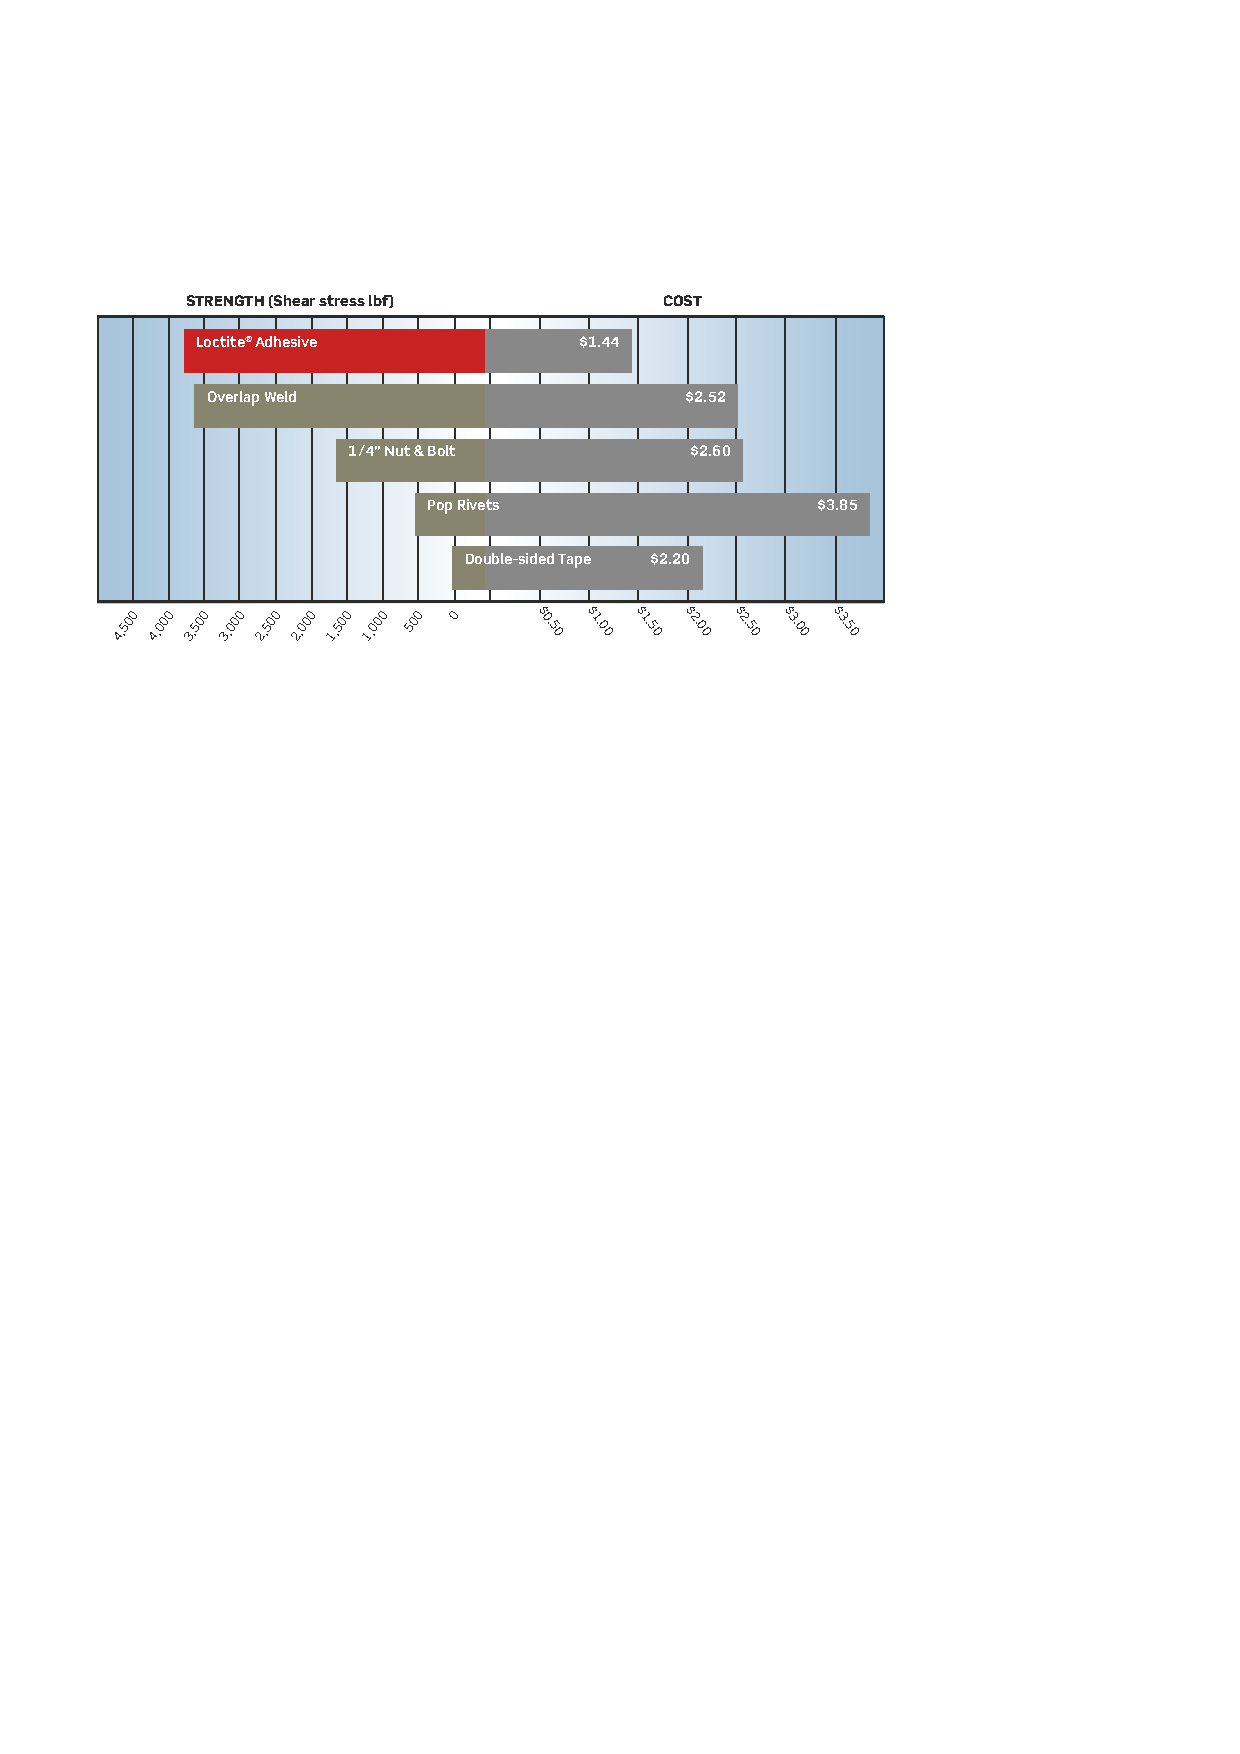
\includegraphics[width=\linewidth]{./figures/IMG_CUTRES/comparison}
	\caption[Qualitative strength and cost comparison of different joining solutions.]{Qualitative strength and cost comparison of different joining solutions. Taken from \cite{superyacht}.}
	\label{fig:comparison}
\end{figure}

As shown in \Cref{fig:comparison}, adhesives are very competitive both in bonding strength and in economical manufacturing costs \cite{superyacht}. In order to check adhesive's suitability for their use in crashworthy elements, this research develops numerical models of adhesively bonded crash boxes subjected to impact loads using finite element models. Information and data present in the literature are used to create and validate these models in order to ensure the accuracy of the results.

\section{Finite element model}
The modeled crash box consists of two adherend cold-formed sheets made of steel that create a tube of square section bonded together with an epoxy adhesive. The joint is practiced on the surface of two flanges on each adherend side. In order to ease the model validation, the crash box geometry was created to reflect those tested by \cite{Peroni2009} and later modeled by \cite{Scattina2011}. In particular, the two sections depicted in \cref{fig:crash_box} are modeled in the present study.

\begin{figure}[htpb]
	\centering
	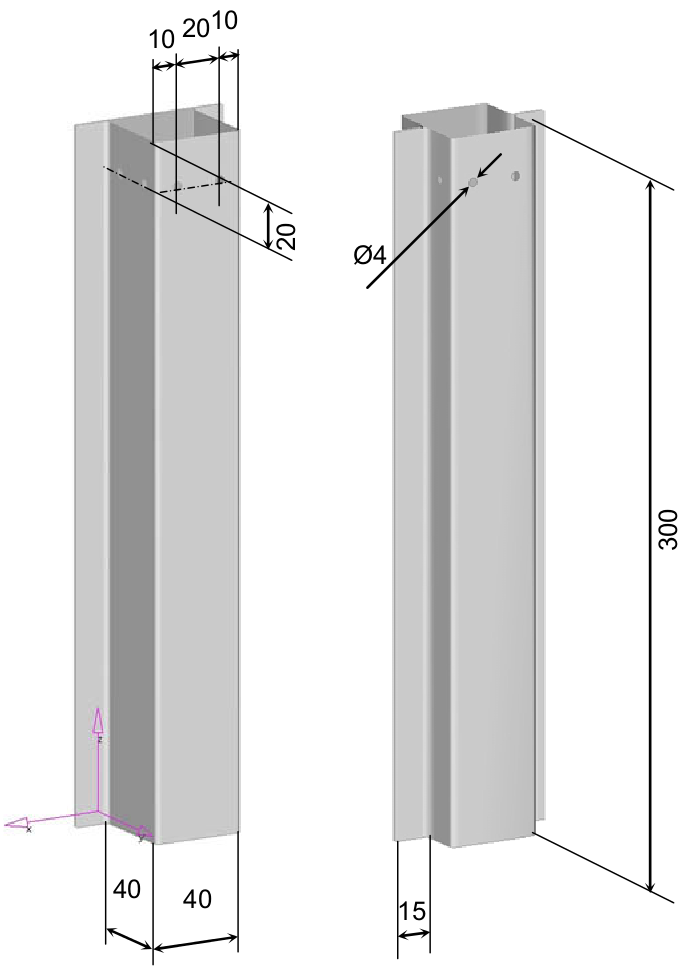
\includegraphics[width=0.5\linewidth]{figures/IMG_CUTRES/medidas_cb}
	\caption{Dimensions of the modeled crash boxes, in millimeters. Taken from \cite{Peroni2009}.}
	\label{fig:crash_box}
\end{figure}

\todo{centrar figuras}

The tube is crushed between two rigid plates, one fixed and the other moving at impact speed. In order to ease the formation of a stable collapse mechanism, a triggering is machined near the front end of the tube. The trigger starts a desired collapse mode in that area.

\subsubsection{Impact conditions} % Speed, etc
\label{sec:impact}

The tube was placed between two circular rigid plates, as it can be seen on \cref{fig:general}, one next to the impact head and the rear one next to the opposite end. The impact plate had a initial separation of $\SI{1}{\mm}$ to avoid simulation problems.

\begin{figure}
	\centering
	\begin{minipage}[b]{.22\linewidth}
		\centering
		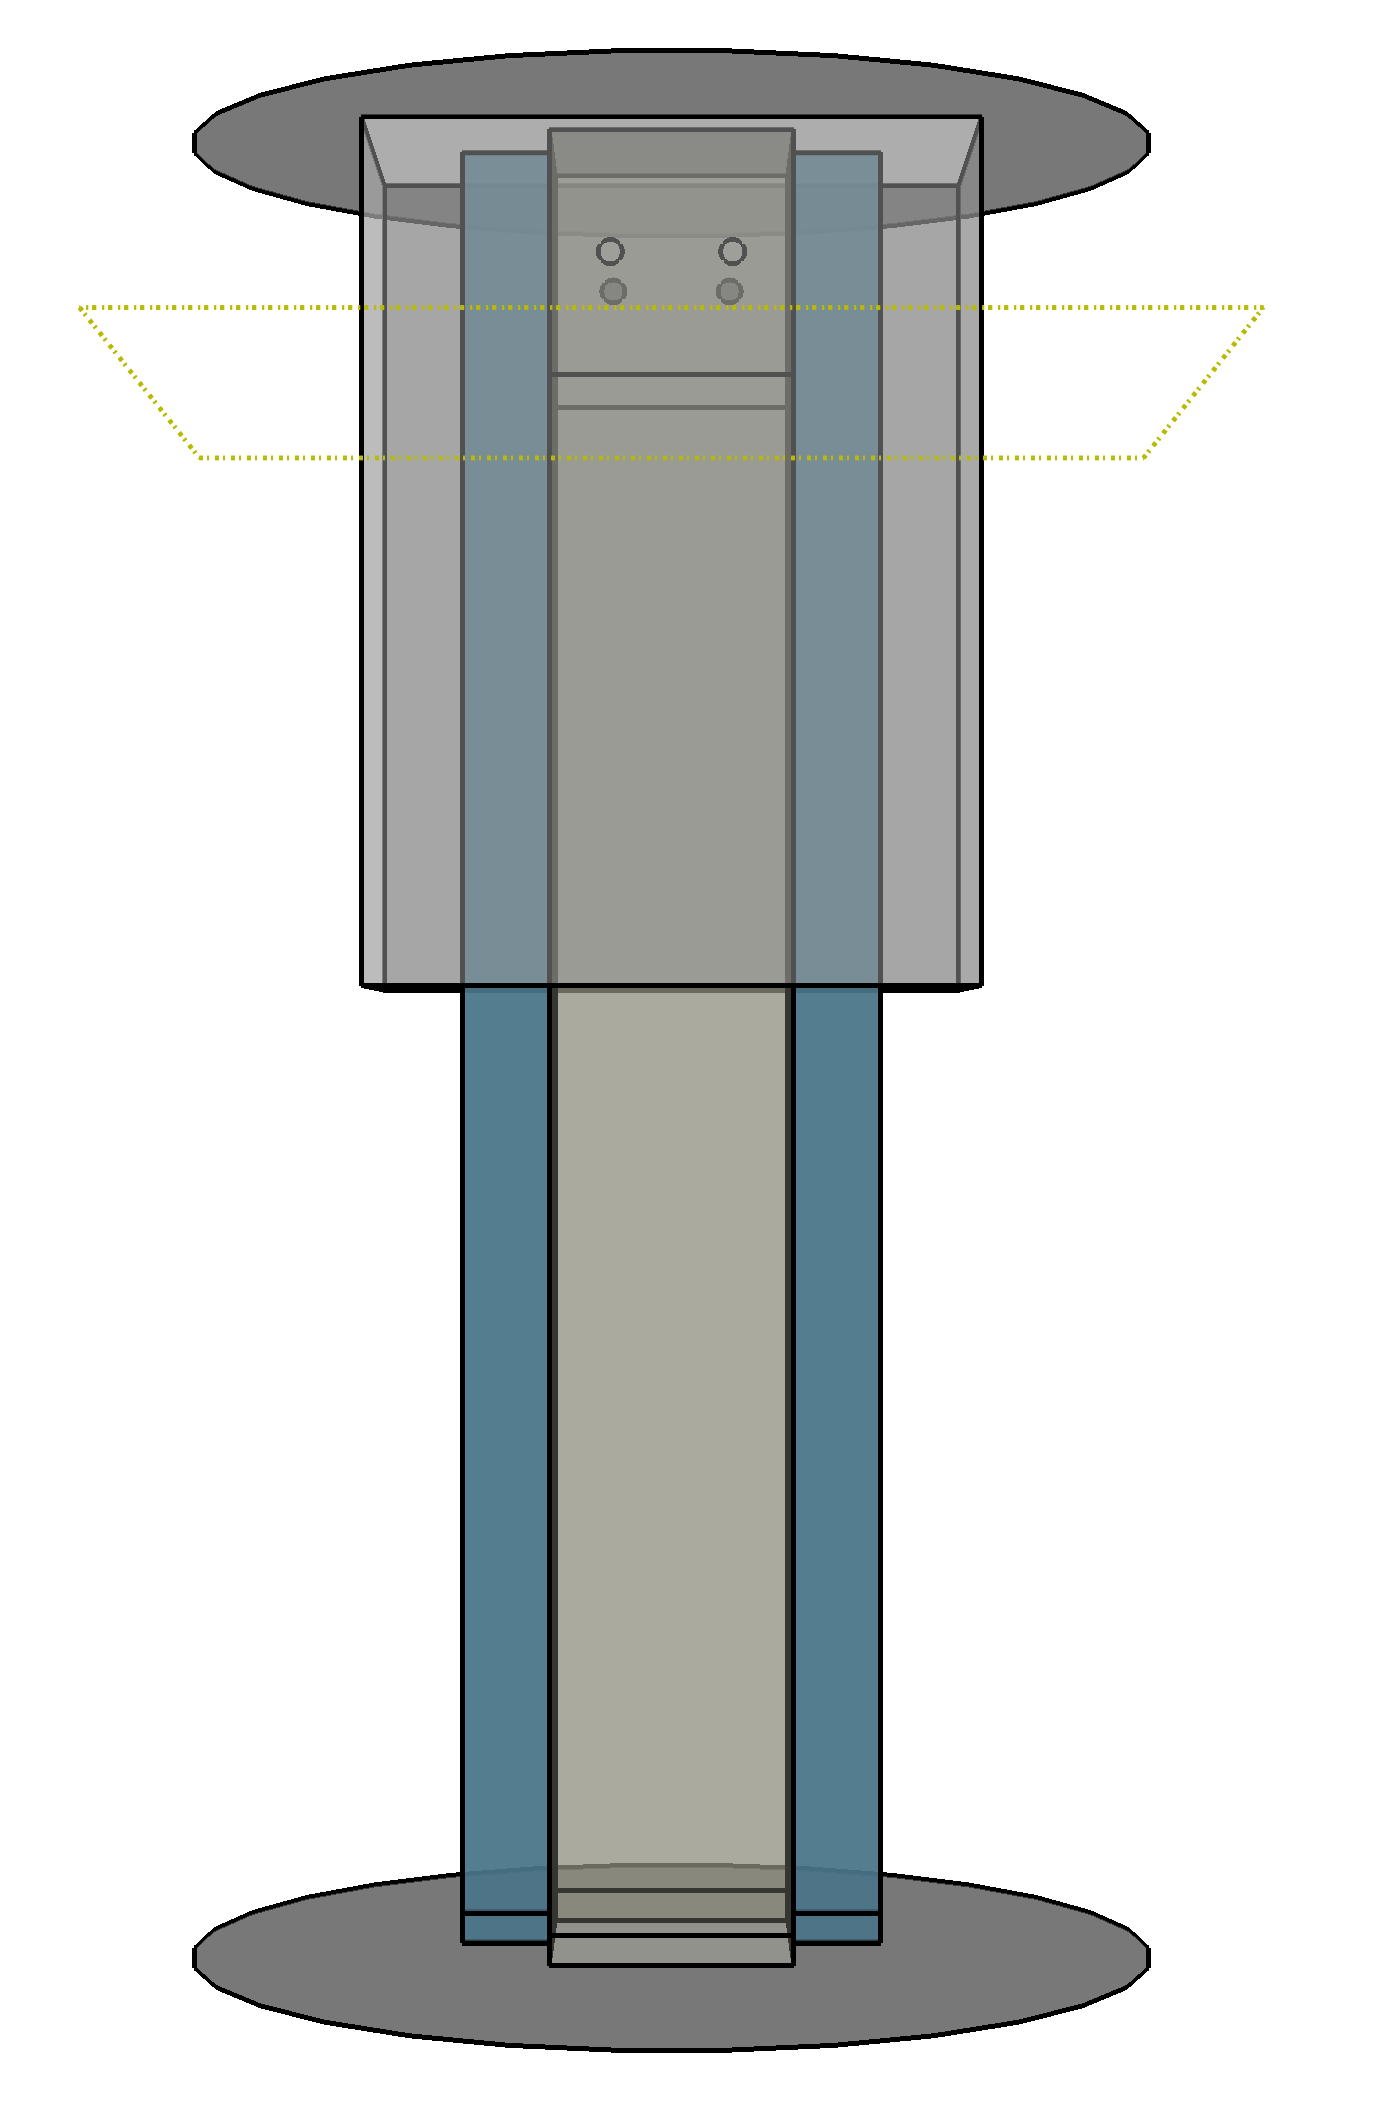
\includegraphics[height=5cm]{figures/IMG_CUTRES/general_transp}
	\end{minipage}
	\quad
	\begin{minipage}[b]{.22\linewidth}
		\centering
		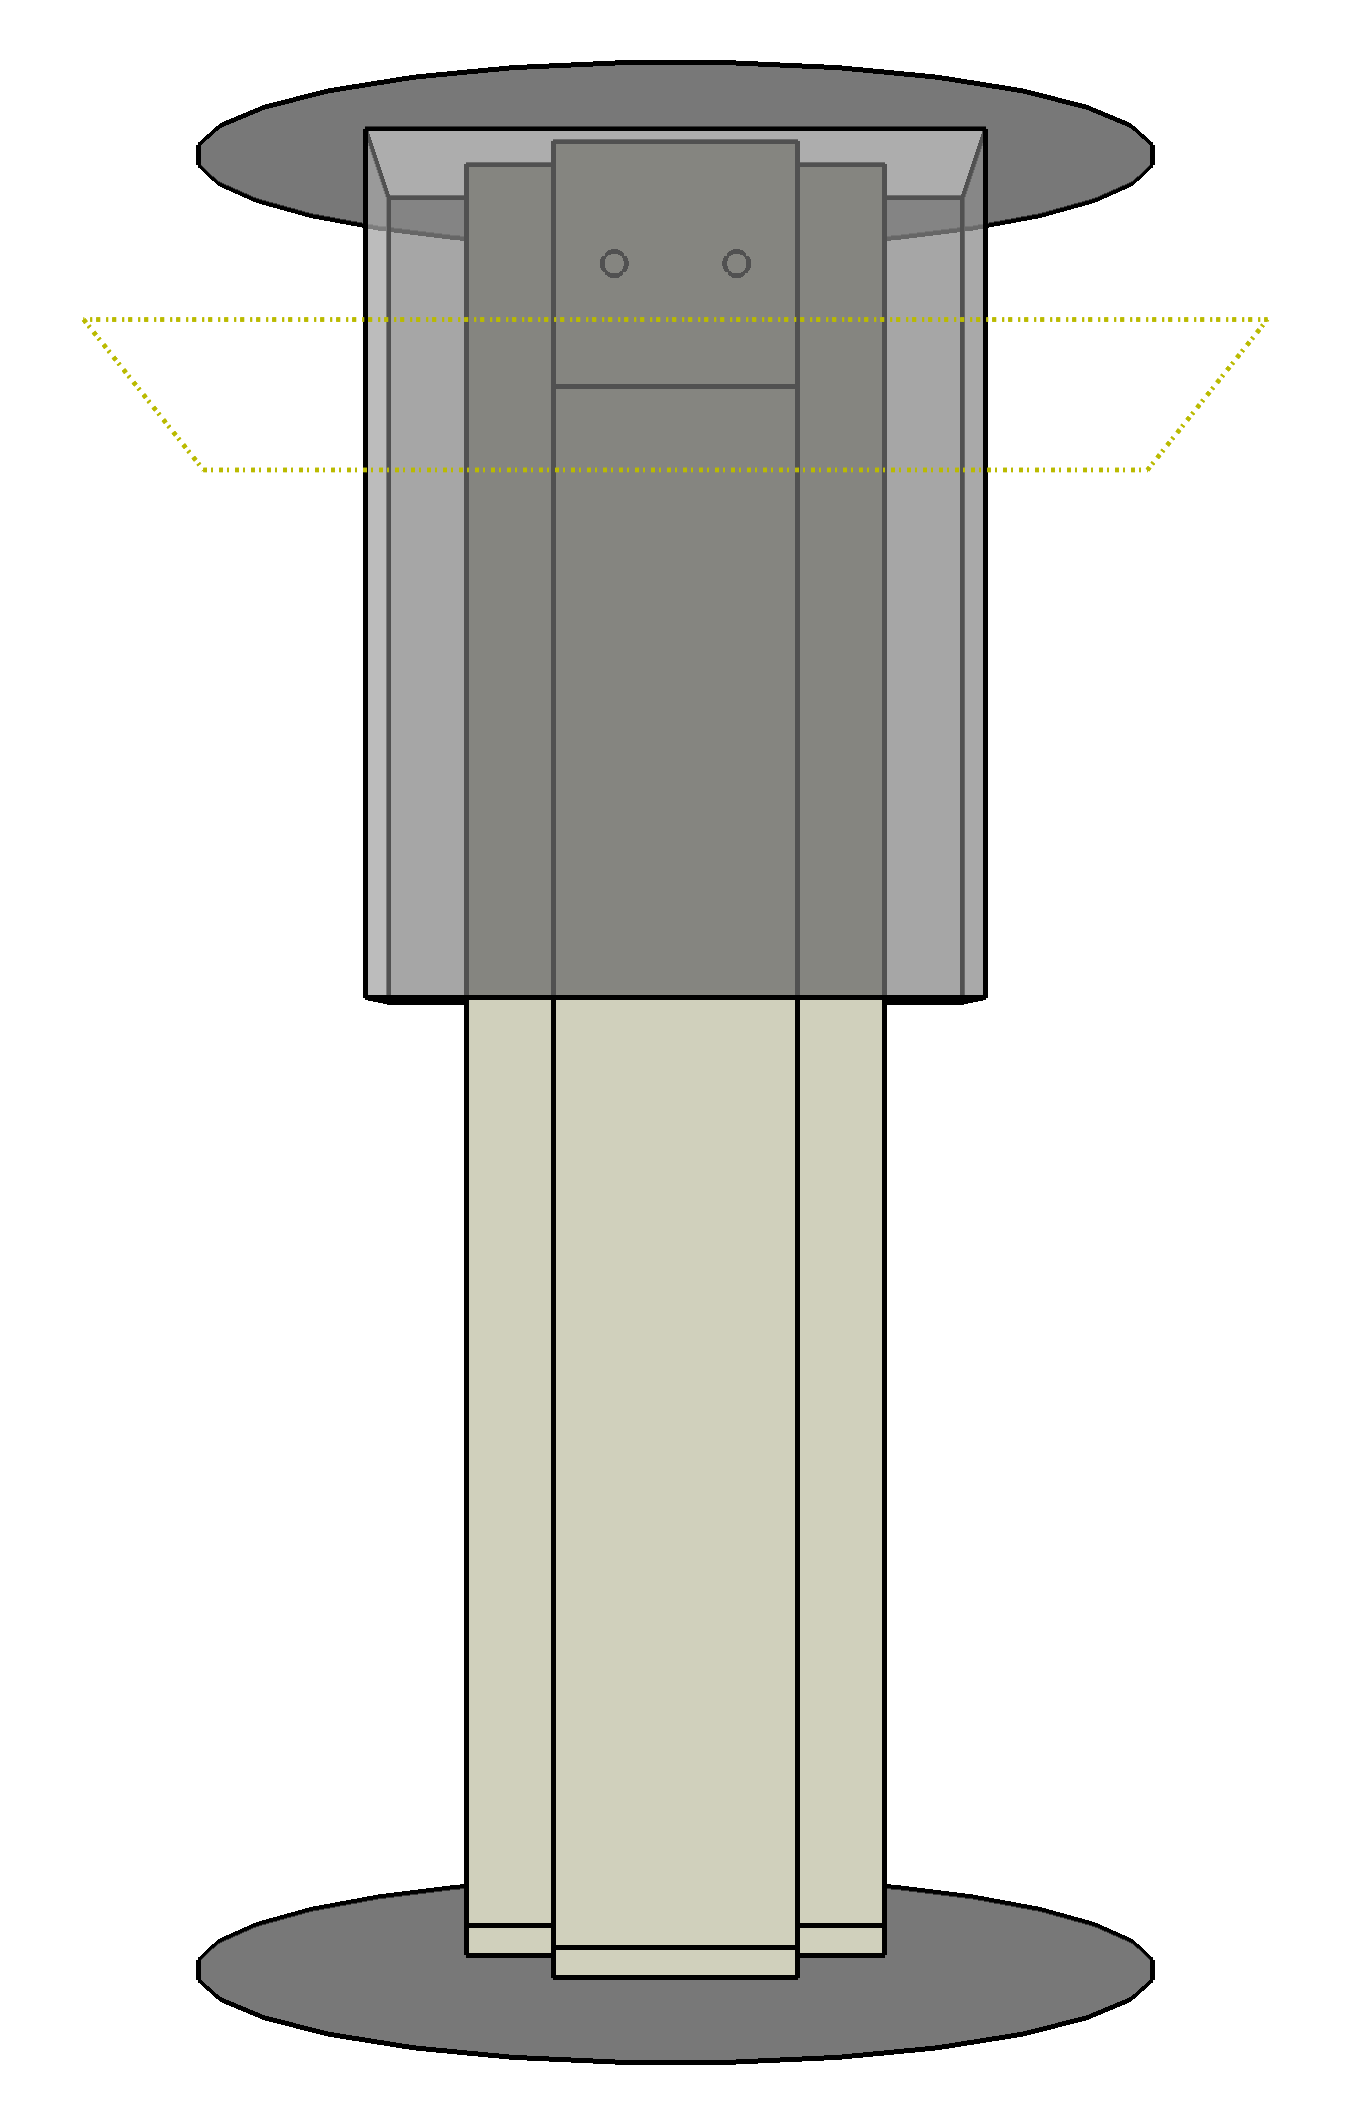
\includegraphics[height=5cm]{figures/IMG_CUTRES/general_rigtransp}
	\end{minipage}
	\quad
	\begin{minipage}[b]{.22\linewidth}
		\centering
		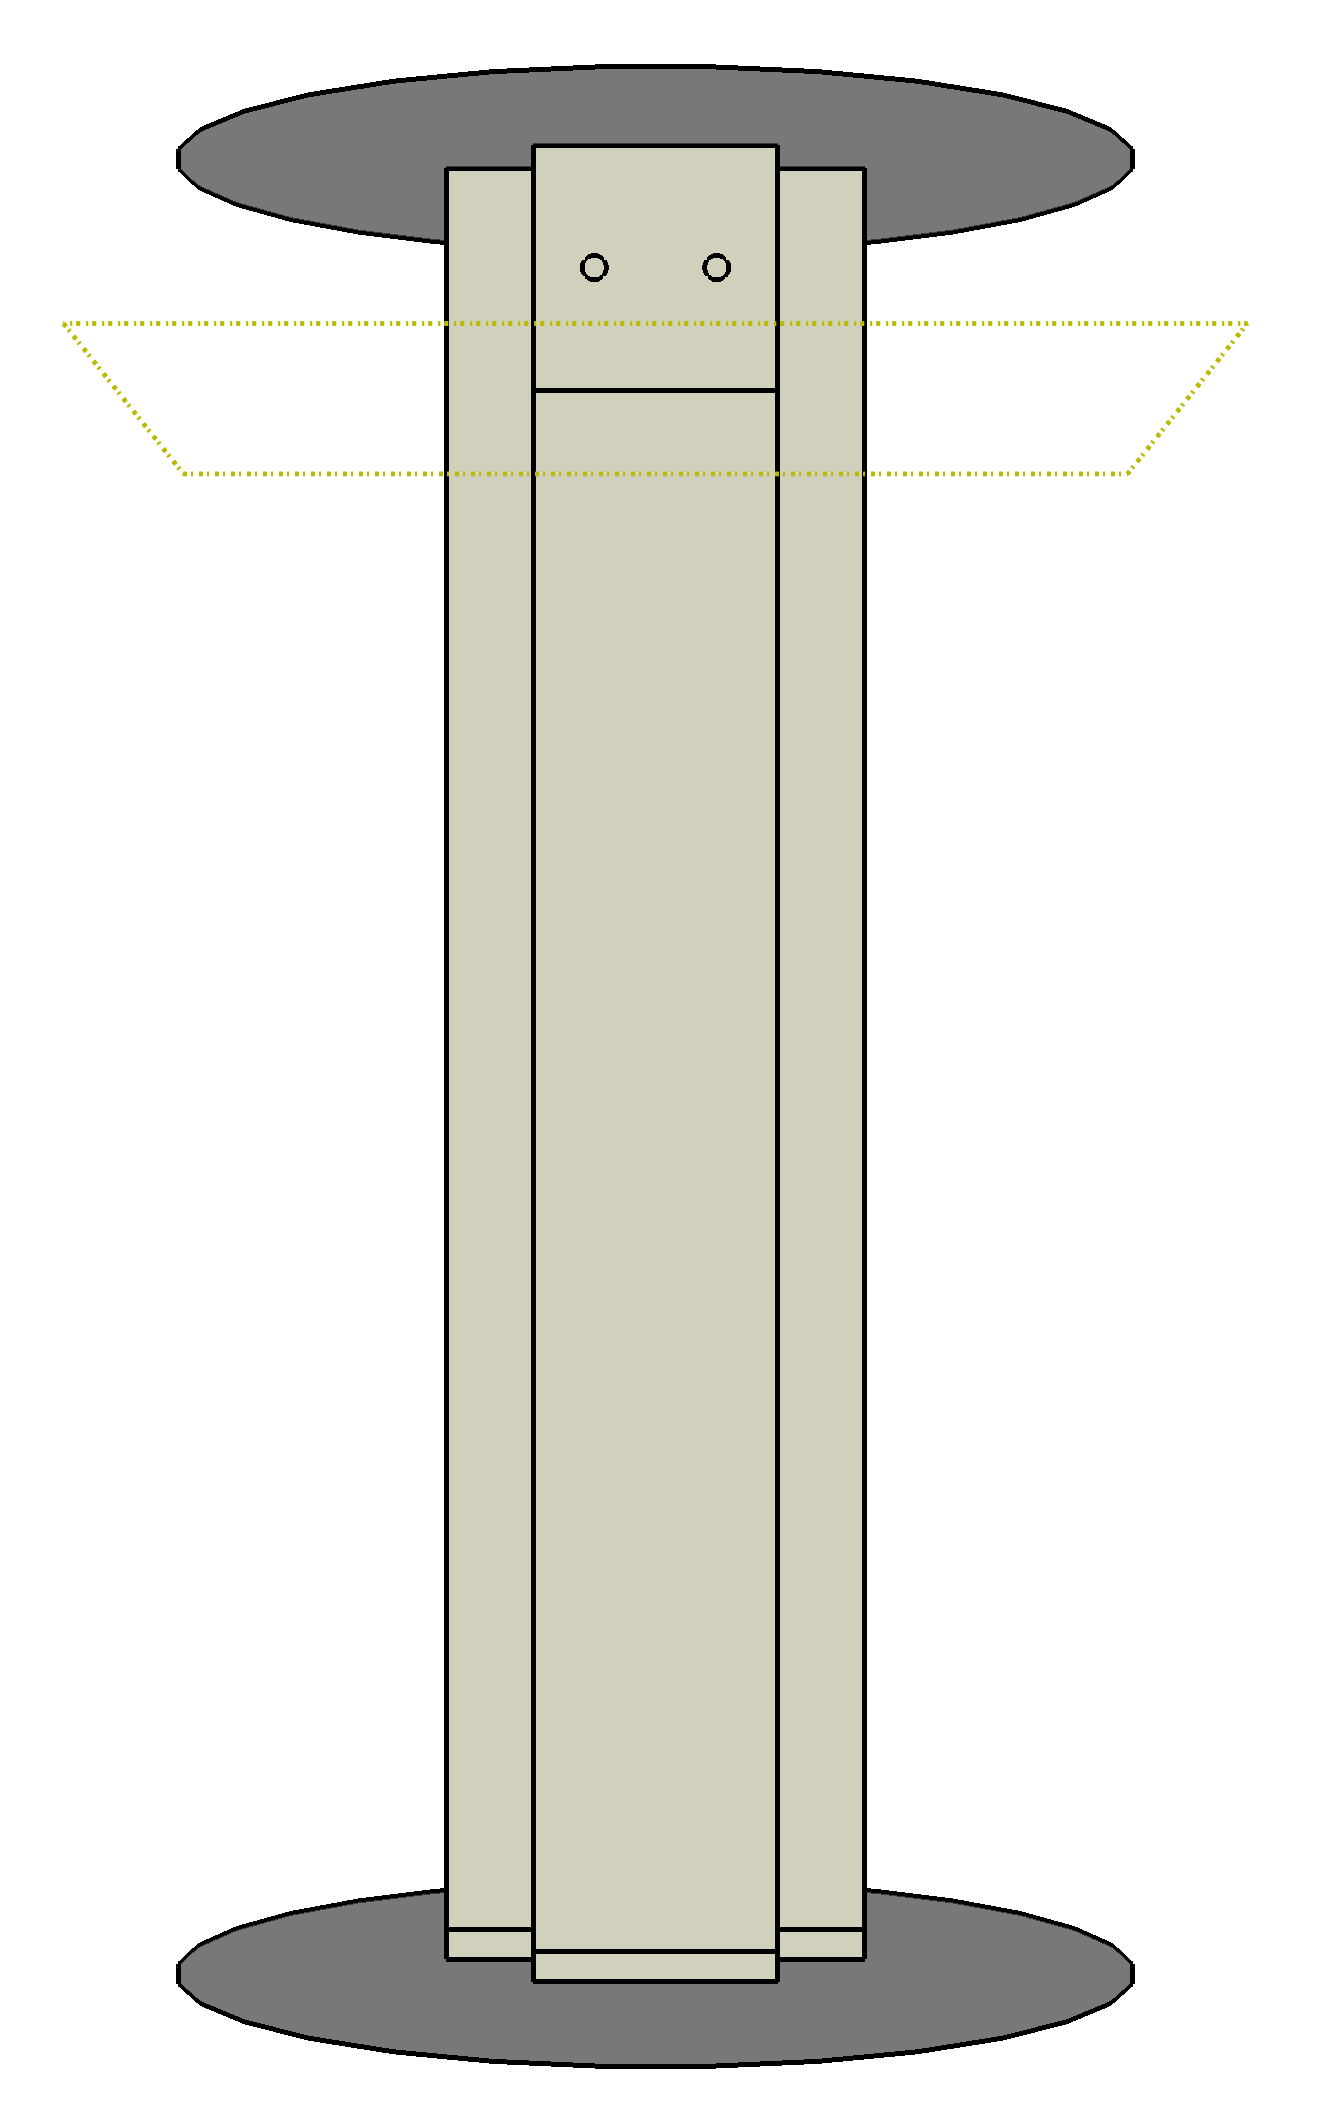
\includegraphics[height=5cm]{figures/IMG_CUTRES/general_noSb}
	\end{minipage}
	\quad
	\begin{minipage}[b]{.22\linewidth}
		\centering
		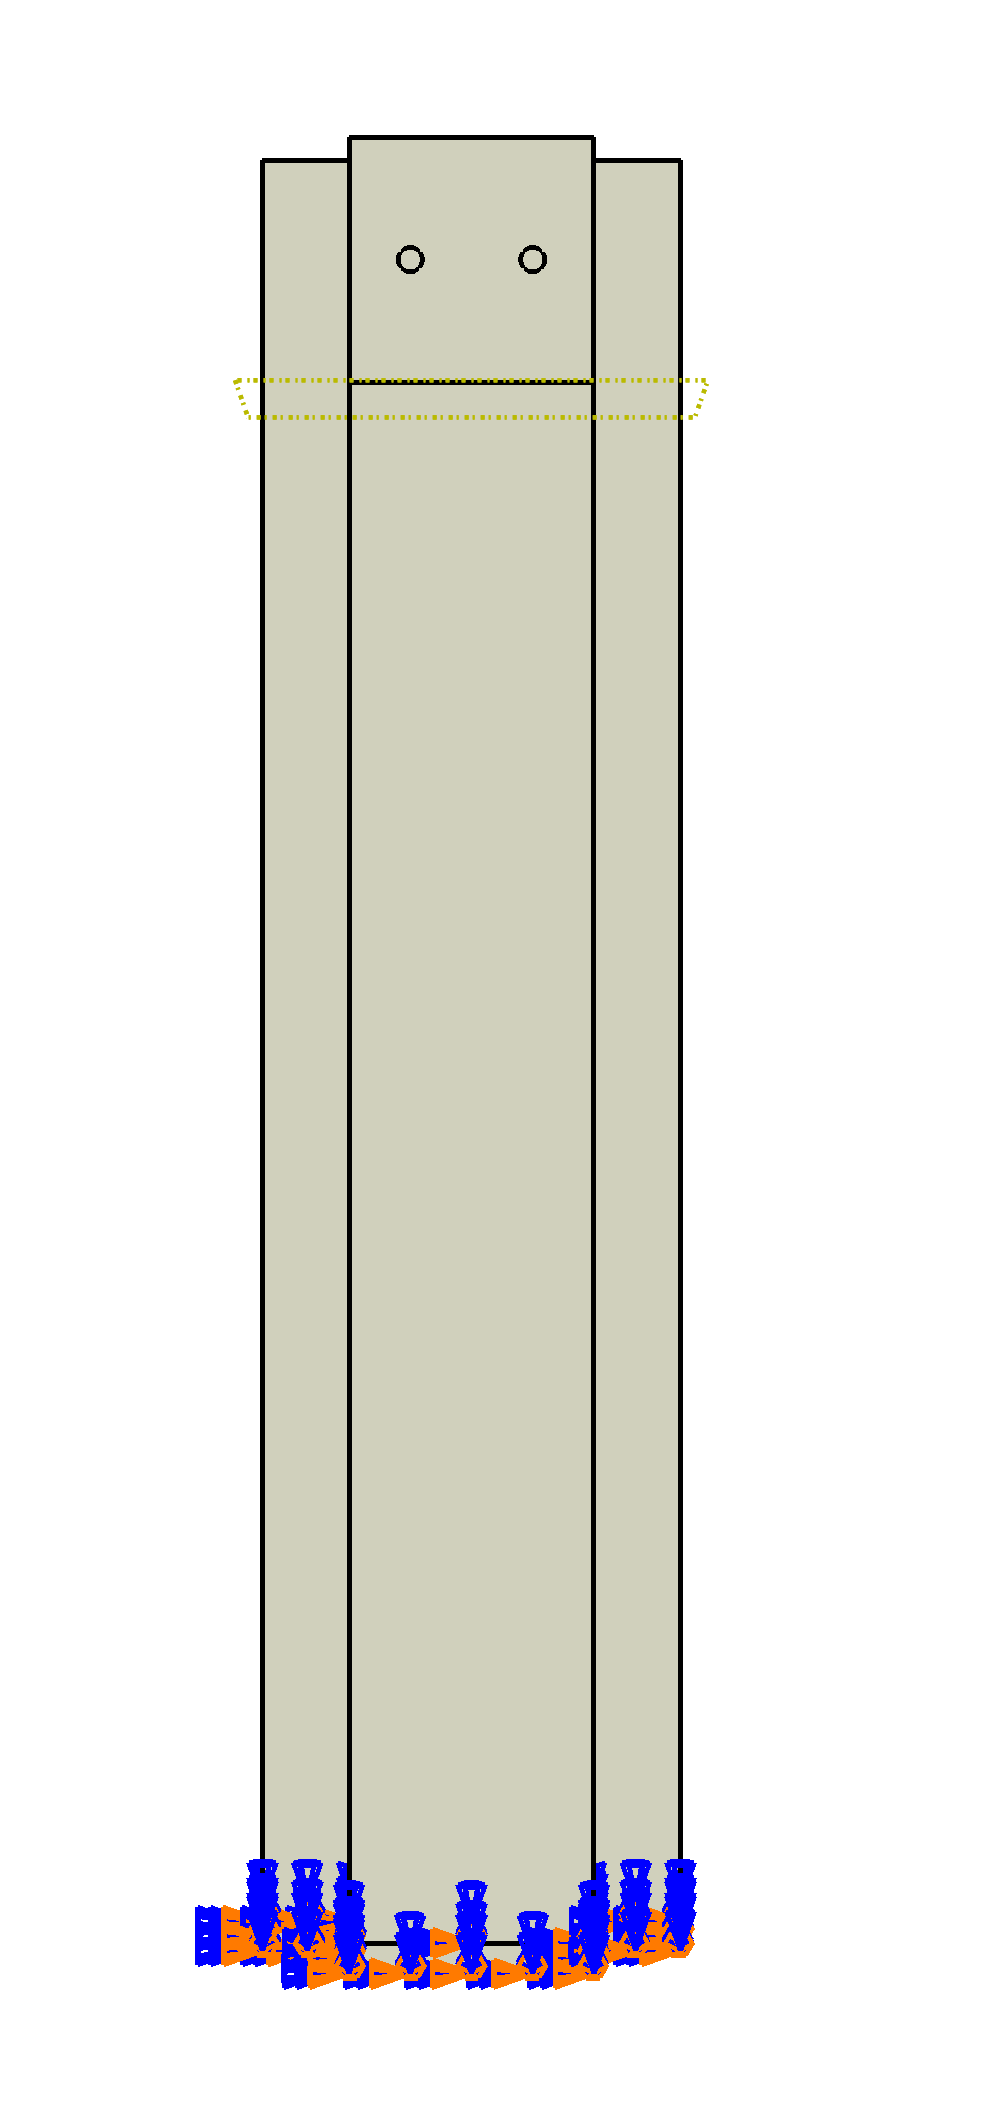
\includegraphics[height=5cm]{figures/IMG_CUTRES/general_encastre}
	\end{minipage}
	\caption[General view of the model.]{General view of the model. Crushing from up to down. From left to right: view with transparency (adhesive in blue); view with rigid parts transparency; view without stabilizing box; view with the fixed part highlighted.}
	\label{fig:general}
\end{figure}

In the bibliography, impact tests are often substituted by quasi-static tests, due to the similarities between both with materials with low sensitivity to strain ratio. References including actual impact tests usually compare both situations \cite{Goglio2008, Peroni2009}, concluding that these two ways of facing this problem are not always equivalent. In this study, a full impact simulation was carried out. The objective is to develop systems that behave in the same manner both in static or low velocity tests and on impact tests.

The impact plate moved during the simulation at $\SI{10}{\m/\s}$ on a total distance equal to half of the total tube's length, resulting in a total analysis time of $\SI{0.015}{\s}$ long. Rotational degrees of freedom were fixed on the frontal plate.

The rear plate had all degrees of freedom restrained. The reaction force that appeared on this point was used to measure Ea, as explained later on (see \cref{sec:Ea}).

The last $\SI{5}{\mm}$ of the crash tube had all degrees of freedom fixed (see \cref{fig:general}), except displacement on the impact direction in order to allow the reaction force measurement commented before. This way, numerical issues due to excesive unrestrained degrees of freedom on the whole tube were prevented.


Peeling problems were found near the impact head end during the development of the study. \cite{Peroni2009} solved this situation by adding two rivets on the bonded flanges at the triggered section in order to avoid excesive debonding on that part of the tube in the initial phases of the impact and, thus, prevent critical situations. In this study, it was substituted by a $\SI{2}{\mm}$-diameter spot-weld point in the same location, as it was a better-known technique for the author and had a very similar effect on the model.

% INSERT IMAGE TO EXPLAIN LOCATION

The spot weld was made up of steel, using its elastic modulus as stiffness and the steel yielding stress on the normal direction as the failure criterion. Several sizes for the spot-weld points were tried up to an average solution which wasn't either too strong to obviate the adhesive's contribution, neither too weak to not prevent the critical failure.


Due to the crushing conditions and the relation between tube length and cross section area, strong difficulties were found in order to achieve stable collapse mechanisms. On their place, tubes diverted from their axis ---other found problems not related with the tube bending are solved through the use of rivets---. Trying to avoid these critical situations, four rigid plates on a rectangular section among the crash tube were added to the model as a stabilizing box.

It has half of the length of the tube and moved together with the impact plate, so the crash tube would end confined between the plates on both ends and the stabilizing box by the end of the simulation. Its section was of $\num{100}\times\SI{60}{\mm}$ and co-centered with the crash box.

The rationale behind this is that in an actual vehicle crash, this device would be among many other vehicle parts ---such as the motor, which is very rigid---, restraining the crash box movements in many directions. It also aims to prevent global buckling problems.

\subsection{Materials}

The model is made up of two different materials, together with several already mentioned ideally rigid parts (see \cref{sec:impact}). The adherends of the tube are made of elastic-plastic steel. The adhesive is an elastic material only considering one normal and two shear directions with a damage formulation.

It must be pointed out that the use of several material with different behaviour formulations including crack formation implies the use of the XFEM. Although it will have some implications in the present section ---and more specifically on \cref{sec:damage}---, the XFEM will be explained afterwards in \cref{sec:xfem} in order to keep some coherence in the explanation.

\subsubsection{Adhesive}
Loctite Hysol 9514 \cite{manufCatalog} was the chosen adhesive for the bonding, for its shown interest by many other authors for structural bonding \cite{Sadowski2010, Scattina2011, SernaMoreno2015}, making it an \textit{a priori} good candidate for the studied application. It is a monocomponent epoxy adhesive which requires heat curing processes in the union cast.

According to \cite{manufCatalog}, the shear strength of the adhesive is $\SI{44}{\MPa}$, although this parameter is subject to variation depending both in cure temperature and time. Dependency can be seen on \cref{fig:catalog_temp}. Given value corresponds to a $\SI{150}{\celsius}$ cure for $\SI{30}{\min}$. The bulk modulus is $\SI{1460}{\MPa}$ and the adhesive's density is $\SI{1.46}{\tonne/\m^3}$ \cite{manufCatalog}.

\begin{figure}
	\centering
	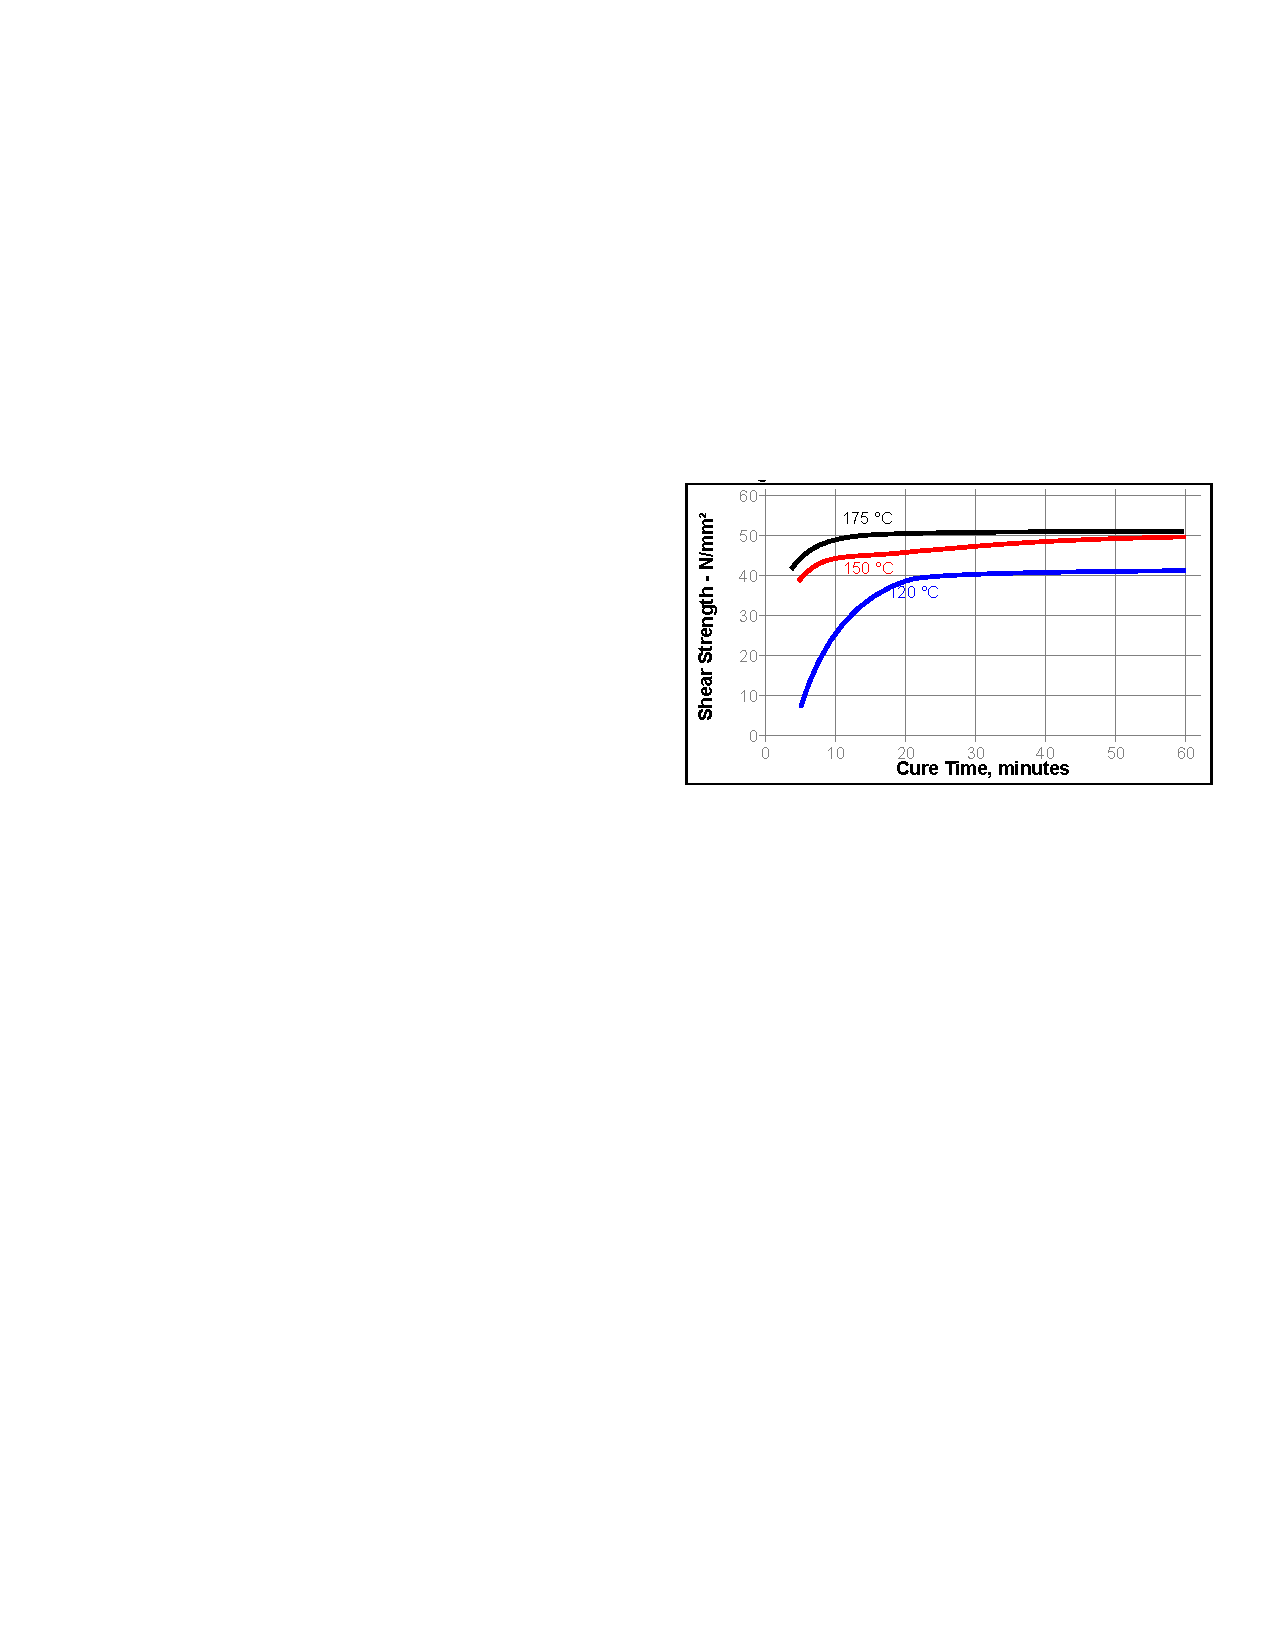
\includegraphics[width=0.7\linewidth]{figures/IMG_CUTRES/catalog_temp}
	\caption[Cure temperature and time dependency of the Loctite Hysol 9514 shear strength.]{Cure temperature and time dependency of the Loctite Hysol 9514 shear strength. Taken from \cite{manufCatalog}.}
	\label{fig:catalog_temp}
\end{figure}


The constitutive behaviour was supposed to be isotropic linear elastic \cite{SernaMoreno2015} up to failure start. An uncoupled traction elastic behaviour \cite{Sadowski2010, Sadowski2011, Scattina2011, Sadowski2014} on 3D cohesive finite elements was the best fit for modelling adhesives \cite{Abaqus613Manual}. \Cref{sec:coh_elem} deepens on the element formulation and properties. \Cref{eq:traction} shows how this model works.

\begin{equation}
\begin{Bmatrix}
t_n \\
t_s \\
t_t \\
\end{Bmatrix}
=
\begin{bmatrix}
E_{nn} & & \\
& E_{ss} & \\
& & E_{tt} \\
\end{bmatrix}
\begin{Bmatrix}
\varepsilon_n \\
\varepsilon_s \\
\varepsilon_t \\
\end{Bmatrix} ;
\label{eq:traction}
\end{equation}
where $t_n$ is the nominal traction in the normal direction; $t_s$ and $t_t$ are the nominal tractions in both shear directions; $E_{nn}$, $E_{ss}$ and $E_{tt}$ are the corresponding stiffnesses; and $\varepsilon_n$, $\varepsilon_s$ and $\varepsilon_t$ are the corresponding nominal strains \cite{Abaqus613Manual}. $E_{ss}$ is considered equal to $E_{tt}$, and this value will be refered as $E_{T}$ onwards. In order to match this nomenclature, $E_{nn}$ will be refered as $E_{N}$.

It is remarked that \cref{eq:traction} relates forces and strains ---not forces and displacements, or stresses and strains, as usual---, implying thus that the value of $E_{N}$ depends on the thickness of the layer. As \cref{eq:traction} refers to each element, the value of $E_{N}$ depends not only on the mentioned geometry, but also on the mesh. In this case, it can be calculated by dividing the elastic modulus, $E$, by the adhesive layer thickness.

This may bring up some problems in those cases in which the adhesive layer has a non-uniform thickness, or very different element lengths between different zones of the material. In our case, elements have fairly uniform in-plane sizes, and the layer has a uniform thickness for the normal direction.

The constitutive model expresed in \cref{eq:traction} is an orthotropic model that only applies in one direction: the stack direction, as refered in \cref{sec:coh_elem}. The reduced adhesive layer thickness makes in-plane compression negligible. Uncoupled behaviour of the elastic components is not considered \cite{Scattina2011}.

\cite{Scattina2011} obtained adhesive stiffnesses through the inverse method, which are summarized in \cref{tab:ads_params}. These same parameters were used in the present study, as their results could be validated with the model.

On the other hand, the elastic modulus in the normal direction can also be calculated using bulk modulus, $K$, provided by \cite{manufCatalog} and a Poisson's modulus, $\nu$, of $\num{0.295}$ \cite{JDiaz}, through the common formula that relates these parameters with the elastic modulus, $E$ in linear elastic mechanics. A similar proceeding would apply for both in-plane shear directions related to the shear modulus, $G$. The values obtained this way would be: $\SI{5.986e9}{\kN/\m^2}$ for $E_{N}$ and $\SI{3.467e8}{\kN/\m^2}$ for $E_{T}$. In spite of that, the values given by \cite{Scattina2011} are finally used.

\begin{table}
	\centering
	\begin{tabular}{llrl}
		Parameter & Description & Value & \\
		
		$E_{N}$ & Stiffness in normal direction & $\num{5e9}$ & $\si{\kN/\m^2}$ \\
		$E_{T}$ & Stiffness in an in-plane direction & $\num{8e7}$ & $\si{\kN/\m^2}$ \\
	\end{tabular}
	\caption[Loctite Hysol 9514 parameters.]{Loctite Hysol 9514 parameters. Taken from \cite{Scattina2011}.}
	\label{tab:ads_params}
\end{table}


% Check other authors here
\Cref{fig:Wu_failure_systems} shows the two possible failure mechanisms that may happen in an adhesive union, as described by \cite{Wu2013}:
\begin{itemize}
	\item Adhesive failure, refered to the contact between different materials, implies the separation of the adhesive from the adherend.

	\item Cohesive failure \cite{Vaidya2006}, refered to the bulk material, means that one piece of adhesive gets teared apart from another, breaking the continuum.
\end{itemize}

\begin{figure}
	\centering
	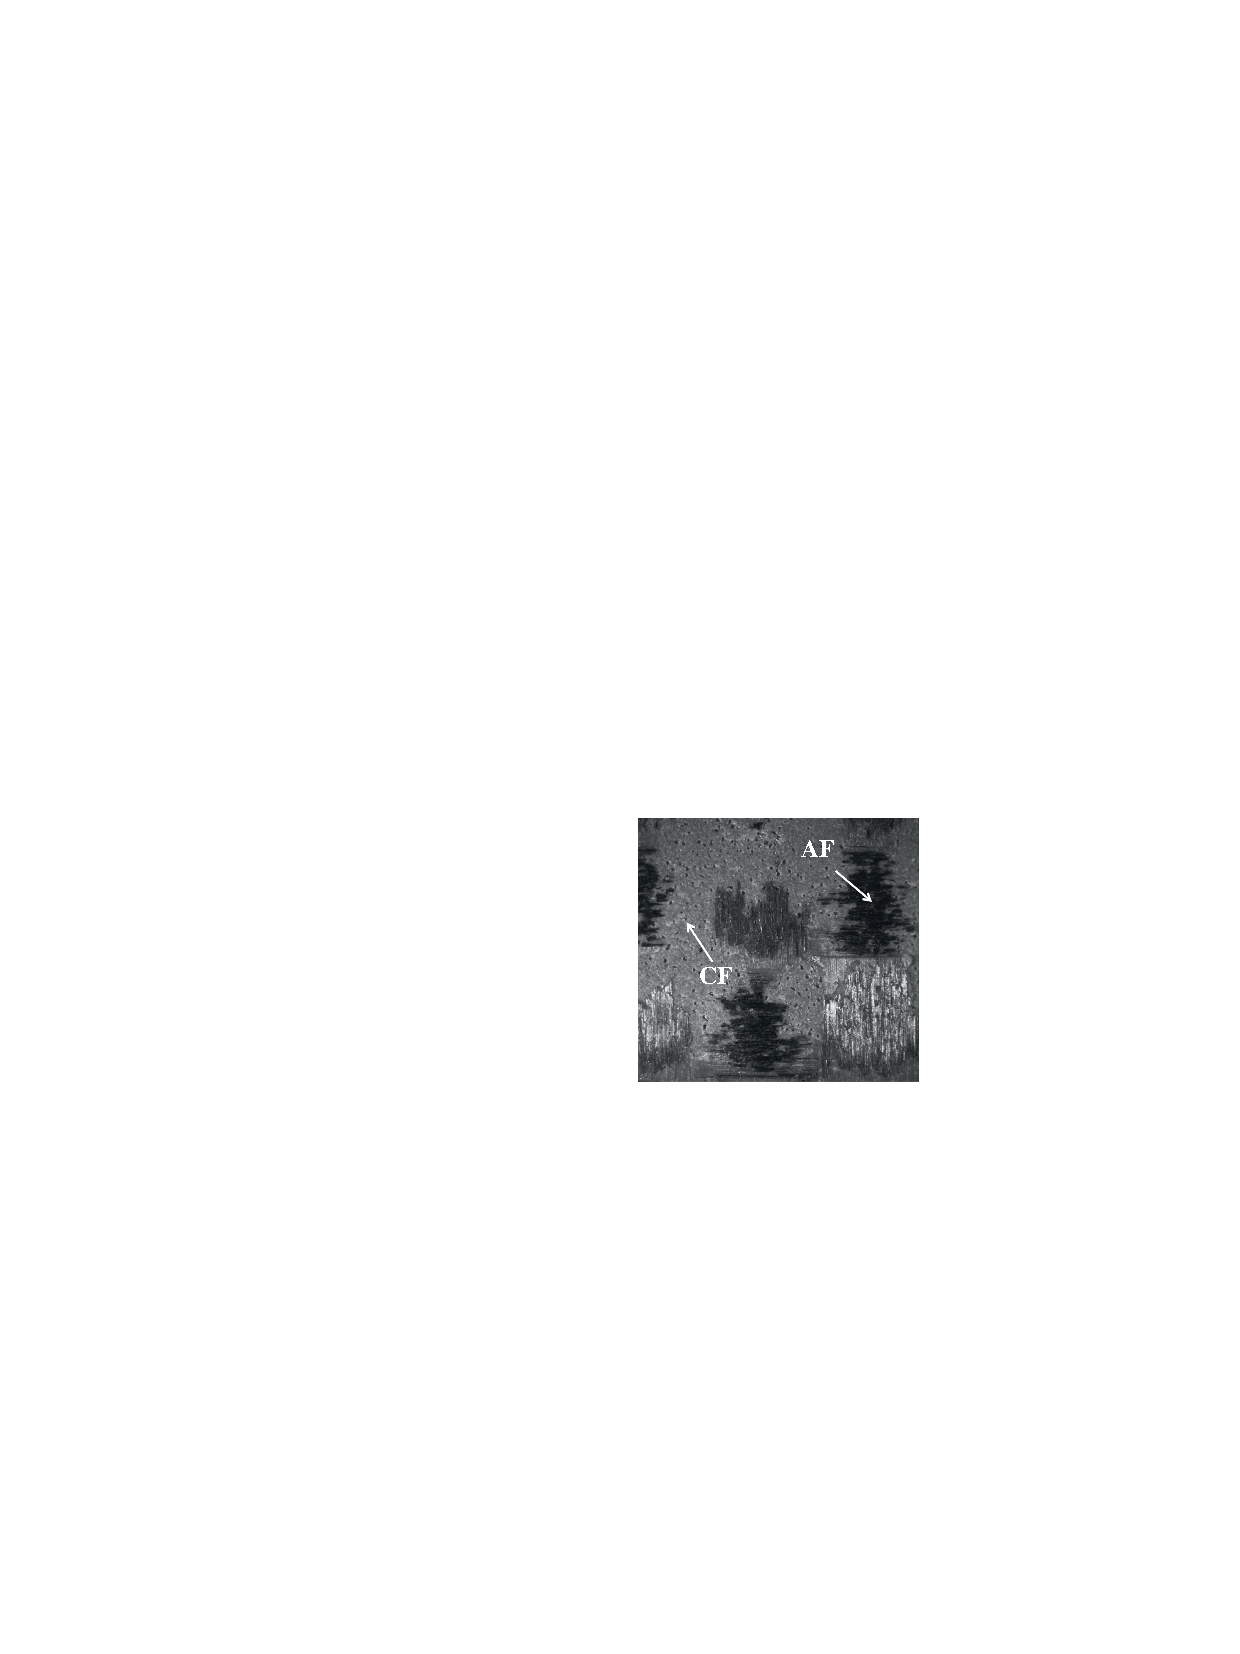
\includegraphics[width=0.7\linewidth]{figures/IMG_CUTRES/Wu_failure_systems}
	\caption[Detail of both possible failure mechanisms of an adhesive union: cohesive failure and adhesive failure.]{Detail of both possible failure mechanisms of an adhesive union: cohesive failure (CF) and adhesive failure (AF). Taken from \cite{Wu2013}.}
	\label{fig:Wu_failure_systems}
\end{figure}

Contact failure modelling ---corresponding to adhesive failure--- resulted in some simulation problems, which are furtherly explained in \cref{sec:coh_elem}. This situation was overcome by including only failure definitions in the bulk material, obviating the contact/adhesive failure as suggested by several authors \cite{Greve2007, Loureiro2010, Sadowski2010, Sadowski2011, Scattina2011, Sadowski2014, SernaMoreno2015}, although the modelled cohesive damage parameters include the effect of both adhesive and cohesive resistance.

The quadratic nominal stress criterion is a widely used damage initiation criterion, defined as
\begin{equation}
\left(\frac{\left<\sigma_{n}\right>}{\sigma_{n}^{0}}\right)^{2} + \left(\frac{\tau_{II}}{\tau_{II}^{0}}\right)^{2} + \left(\frac{\tau_{III}}{\tau_{III}^{0}}\right)^{2} = 1 ;
\label{eq:quads}
\end{equation}
where $\sigma_{n}^{0}$, $\tau_{II}^{0}$ and $\tau_{III}^{0}$ represent the pure mode loading threshold stresses for each direction. The out-of-plane value, $\sigma_{n}^{0}$, was set to $\SI{42.5}{\MPa}$ \cite{Scattina2011}, which corresponds to the peeling failure stress for steel. Note that Macaulay brackets indicate that compression is not considered in failure initiation. Both in-plane values, $\tau_{II}^{0}$ and $\tau_{III}^{0}$, were set to $\SI{130}{\MPa}$ \cite{Scattina2011}. These values are also included in \cref{tab:ads_dmg_params}. % ref to catalog?

\begin{table}
	\centering
	\begin{tabular}{llrl}

		

		Parameter & Description & Value & \\

		

		$G_{Ic}$ & Energy release rate for mode I & $\num{2028}$ & $\si{\J/\m^2}$ \\
		$G_{IIc}$ & Energy release rate for mode II & $\num{11853}$ & $\si{\J/\m^2}$ \\
		$\sigma_{n}^{0}$ & Peak traction in normal direction & $\num{130}$ & $\si{\MPa}$ \\
		$\tau_{II}^{0}$ & Peak traction in tangential direction & $\num{42.5}$ & $\si{\MPa}$ \\

		

	\end{tabular}
	\caption[Summary of Loctite Hysol 9514 damage parameters.]{Summary of Loctite Hysol 9514 damage parameters. Taken from \cite{Scattina2011}.}
	\label{tab:ads_dmg_params}
\end{table}

As long as the condition exposed in \cref{eq:quads} is not satisfied, the adhesive layer behaves elastically. Once the condition gets satisfied, damage starts and a degradation in stiffness can be appreciated following the especified damage evolution model, being thus a case of LEFM, as the traction behaviour is also linear and no yielding takes place at any point.

These three failure modes are represented in \cref{fig:wikipedia_failure_modes} in a qualitative manner in order to give an idea of their geometrical features:
\begin{itemize}
	\item Mode I, or opening mode: produced by a tensile stress normal to the plane of the crack.

	\item Mode II, or sliding mode: originated by a shear stress acting in the crack plane, but perpendicularly to the crack front.

	\item Mode III, or tearing mode: caused by a shear stress on the crack plane and parallel to the crack front.
\end{itemize}

\begin{figure}
\centering
\begin{minipage}[b]{.3\columnwidth}
	\centering
	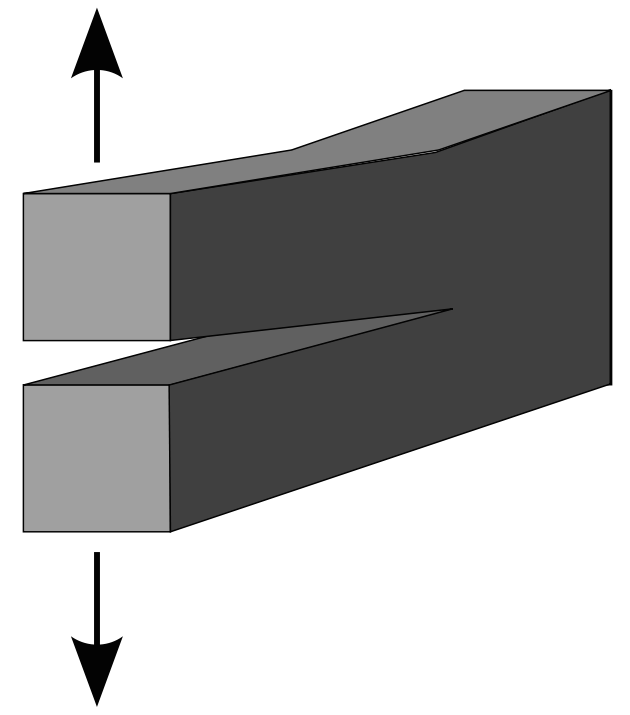
\includegraphics[width=\columnwidth]{figures/IMG_CUTRES/wikipedia_failure_modes_1}
			Mode I:	Opening
\end{minipage}
\hfill
\begin{minipage}[b]{.3\columnwidth}
	\centering
	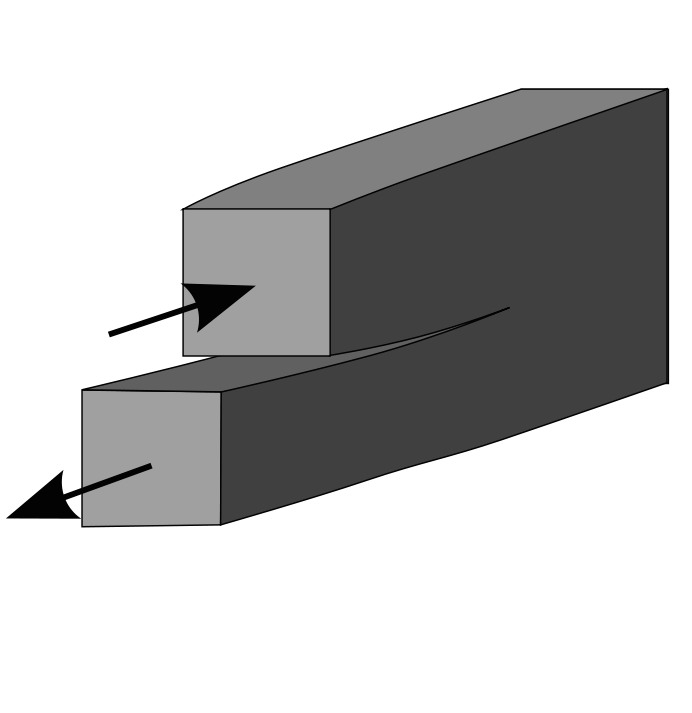
\includegraphics[width=\columnwidth]{figures/IMG_CUTRES/wikipedia_failure_modes_2}
			Mode II: Sliding shear
\end{minipage}
\hfill
\begin{minipage}[b]{.3\columnwidth}
	\centering
	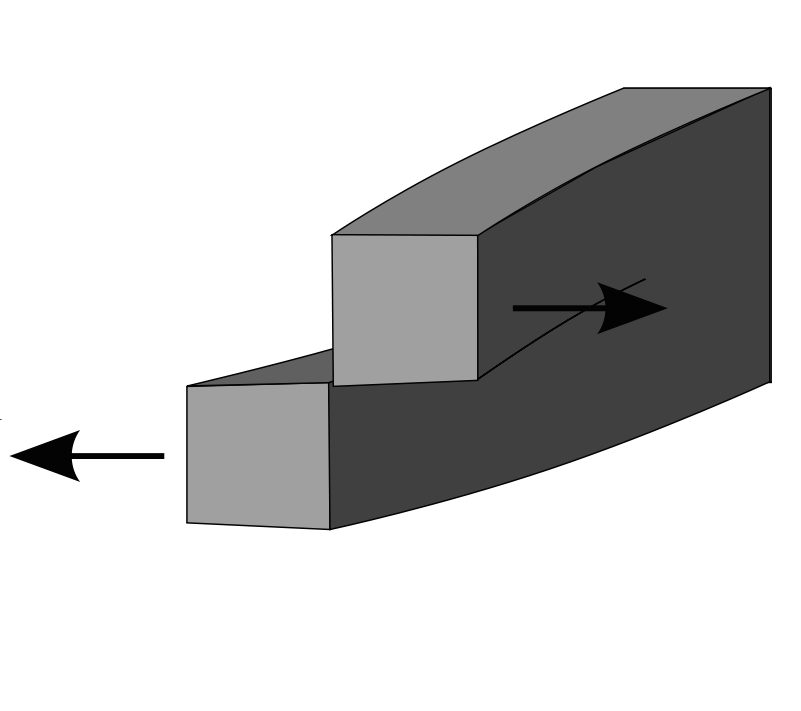
\includegraphics[width=\columnwidth]{figures/IMG_CUTRES/wikipedia_failure_modes_3}
			Mode III: Tearing shear
\end{minipage}
	\caption[Schematic view of the three failure modes.]{Schematic view of the three failure modes. Taken from \cite{wiki_fracture_modes}.}
	\label{fig:wikipedia_failure_modes}
\end{figure}

XFEM-based LEFM require a pre-existing crack in the model or some nucleation formulation that governs its propagation \cite{Abaqus613Manual}. As the crack's initial localization and direction is not previously known, the VCCT criterion is used, which consists on correlating the displacement energy to the suffered damage. This technique can be applied in brittle crack formation, which is the case, as no yielding happens before damage or failure.

For this particular case, the VCCT formulation was set as a fracture energy power law \cite{Loureiro2010, Sadowski2010, Sadowski2011, Sadowski2014, SernaMoreno2015}, as the given by \cref{eq:fracture_energy}.

\begin{equation}
\left(\frac{G_{I}}{G_{Ic}}\right)^{\alpha}+\left(\frac{G_{II}}{G_{IIc}}\right)^{\alpha}+\left(\frac{G_{III}}{G_{IIIc}}\right)^{\alpha}=1 ;
\label{eq:fracture_energy}
\end{equation}
where $G_{Ic}$ corresponds to the critical fracture energy required to cause failure in mode I (out-of-plane direction), and being $G_{IIc}$ and $G_{IIIc}$ the values for mode II and III, respectively, which correspond to both shear directions. The critical fracture energy for the Loctite Hysol 9514 in the normal direction is $\SI{2028}{\J/\m^2}$ \cite{Scattina2011}. It was considered that the adhesive had no preferential directions for tangential failure, meaning $G_{IIc}$ was equal to $G_{IIIC}$, and being the fracture energy equal to $\SI{11853}{\J/\m^2}$ \cite{Scattina2011}. These values are also depicted in \cref{tab:ads_dmg_params}. The exponent $\alpha$ was considered equal to $\num{2}$ \cite{Loureiro2010, Sadowski2010, Sadowski2011, Sadowski2014, SernaMoreno2015}.

In addition, relating this equation to \cref{eq:quads} a stress increase in one mode ---initially suppossed on the limit just before damage progression--- provokes stiffness loss in every mode involved in \cref{eq:fracture_energy}.

Once damage has started, according to this model, fracture energy is released as damage progresses reducing material stiffness. If unloaded, the material would behave elastically again with degraded properties until damage criterion is accomplished again. \Cref{fig:damage_evo2D} illustrates this behaviour for a simplified 2D case.

\begin{figure}
	\centering
	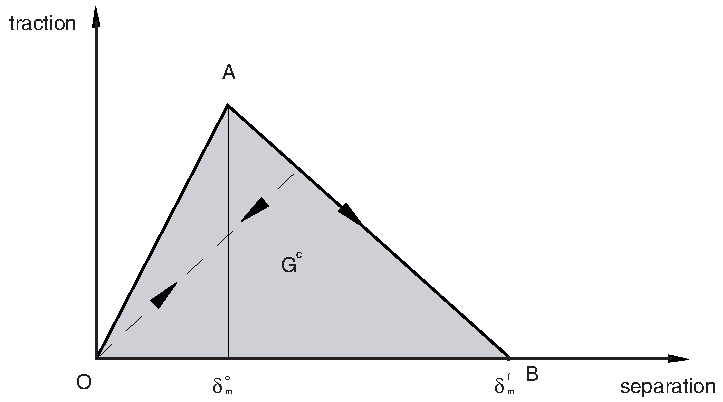
\includegraphics[width=0.7\linewidth]{figures/IMG_CUTRES/damage_evolution_manual.pdf}
	\caption[Damage evolution representation for a 2D case.]{Damage evolution representation for a 2D case. Taken from \cite{Abaqus613Manual}.}
	\label{fig:damage_evo2D}
\end{figure}

Figure \ref{fig:damage} represents the whole damage model, including damage initiation and the fracture energy, which corresponds to the area beneath the curve.

\begin{figure}
	\centering
	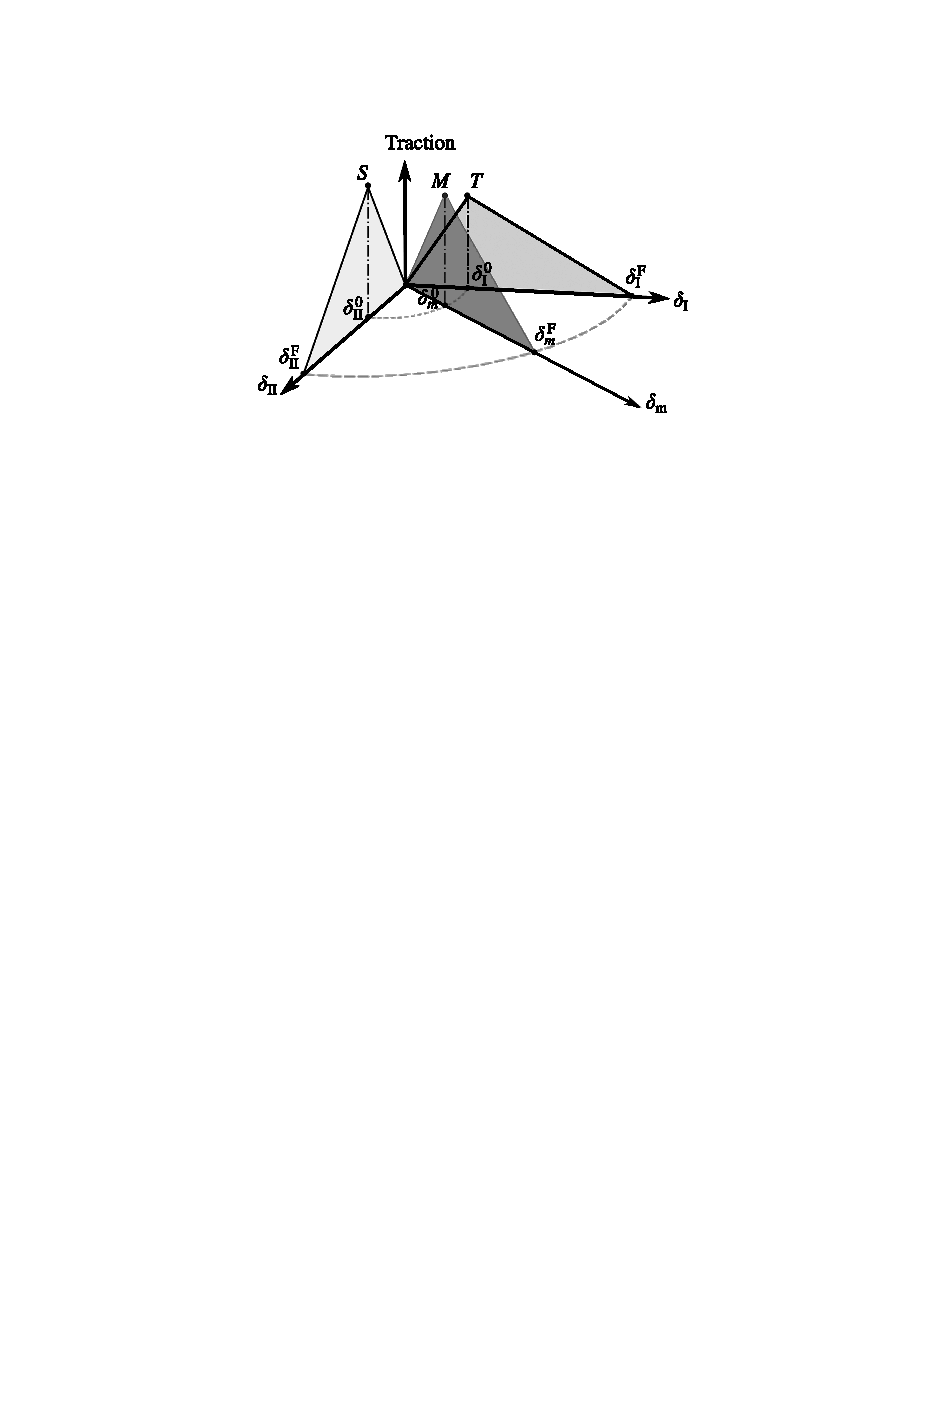
\includegraphics[width=0.7\linewidth]{figures/IMG_CUTRES/scattina_quads}
	\caption[Damage model representation.]{Damage model representation. Traction represents the load; $\delta$, the displacement ($\varepsilon$ in this study); $S$ and $T$, the maximum load in two different modes ($\sigma_{n}^{0}$, $\tau_{II}^{0}$ or $\tau_{III}^{0}$), corresponding to damage initiation, which takes place at $\delta^0$; and $\delta_m$, the displacement in the mixed-mode loading. Taken from \cite{Scattina2011}.}
	\label{fig:damage}
\end{figure}

\subsubsection{Adherends}

In order to make the model comparable to the experiments carried out by \cite{Peroni2009}, steel was chosen for the adherends. In the present study, it is defined as an isotropic elastic-plastic material, with a density of $\SI{7.85}{\tonne/\m^3}$.

The elastic branch of the adherend stress-strain curve is defined as linear, with an elastic modulus of $\SI{200}{\GPa}$ and a Poisson ratio of $\num{0.3}$. It is followed by a perfectly plastic branch starting at $\SI{190}{\MPa}$ up to $\SI{1140}{\MPa}$, which is considered total failure of this material. This way, some strain is allowed during the plastic branch in order to avoid numerical issues, as it can be seen on \cref{fig:steel}.

\begin{figure}
	\centering
	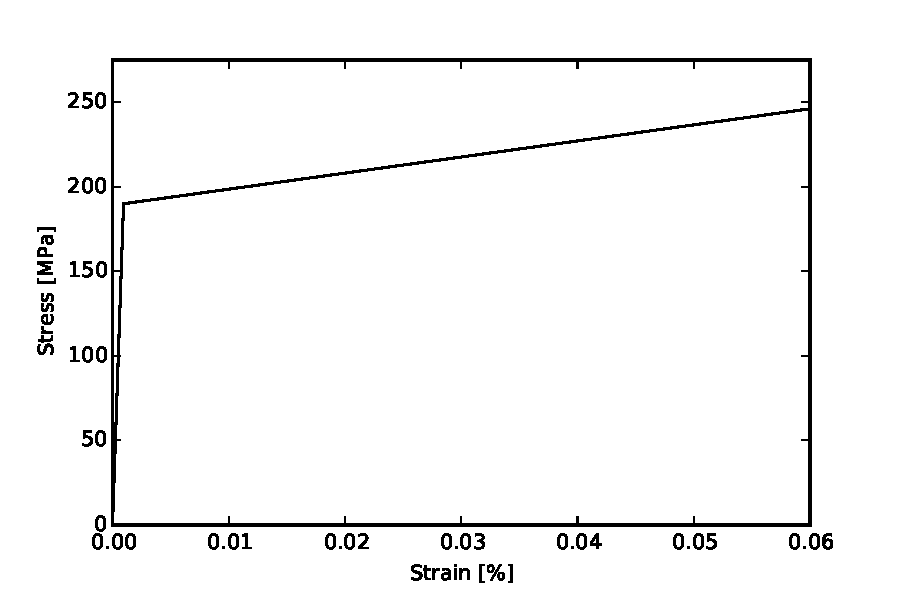
\includegraphics[width=0.7\linewidth]{figures/IMG_CUTRES/steel}
	\caption{Steel stress-strain curve up to $\num{0.0006}$ strain rate.}
	\label{fig:steel}
\end{figure}

It was supposed that the plastic branch of the steel would not develop enough to make necessary to take into account great kinematic harding effects, and was thus obviated.

\subsubsection{Interaction}

A general contact interaction was considered among all surfaces, including contact with themselves. Hard contact was considered on the normal direction, which implies that no penetration between surfaces may occur in case of contact. Models with both rough and frictionless contact were considered on the tangential directions, meaning that no slip may take place or that slip may happen without any resistance, respectively.

Frictionless models resembled those ones with penalty tangential behaviour with minor variations, specially on the last phases of the impact. This may be due to the absence of strong normal forces between adherends and with little tangential load. An exception is found in the tube end in contact with the impact plate, where tangential loading is more important, as the differences in the results point out.

\subsection{Computational and numerical considerations}
% Include computational time

\subsubsection{Hardware and software}

The finite element package Abaqus is used in this research, on is version 6.13 \cite{Abaqus613Manual} running on a high performance computing cluster running CentOS Linux distribution.

Abaqus calculation kernel ---Abaqus/Explicit in this case--- works parallelized on several processors in the cluster. Loop parallelization uses a shared memory paradigm and domain parallelization is based on a distributed memory model with message passing. TcT may vary between similar jobs depending on the processor capabilities. Due to this, only approximations to TcT are given, instead of precise values.

Jobs running on loop parallelization over $16$ cores took about $\SI{8}{\hour}$ to finnish, which could be reduced to about $\SI{1}{\hour}$$\SI{15}{\minute}$ if mass scaling was applied. Domain paralelization turned out to be inefficient in this case due to network performance.


\subsubsection{Model parametrization}
\label{sec:script}

Excepting some details added in the last phases of the development of the present study, the whole model has been parametrized, making use of the Python interpreter integrated in Abaqus. This will allow model optimization in future phases of development. The parametrization code includes:

\begin{itemize}
	\item Geometrical parameters, including: tube length, bonding flanges dimension, adhesive and adherend thicknesses, among others.

	\item Impact conditions, such as speed or crush length.

	\item Two cross sections: square and hexagonal.

	\item Meshing parameters.

	\item Possibility to have a material library, although it is not used due to the lack of validated models.

	\item Optional tube fill with solid material and/or inner free plates.

	\item Different contact formulations.
\end{itemize}

A flowchart explaining the model creation process of the code is depicted in \cref{fig:flow}. Complementary scripts were also developed for its work within the cluster and for its optimization using the Dakota optimization software package \cite{dakota}.

\begin{figure}
	\centering
	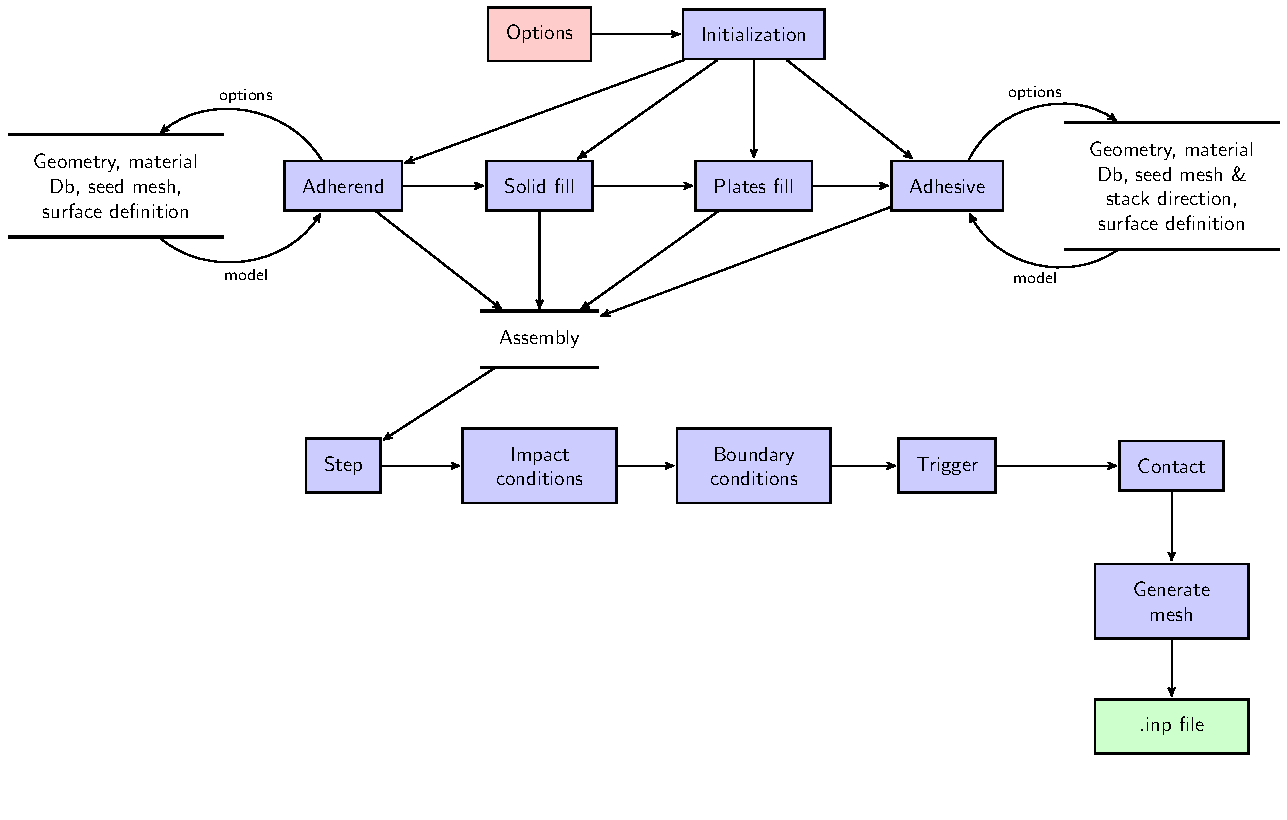
\includegraphics[width=.95\linewidth]{flowchart/flow}
	\caption[General structure of the parameterized code.]{General structure of the parametrization code. Straight arrows imply both chronological order and data dependency.}
	\label{fig:flow}
\end{figure}


\subsubsection{On the XFEM and the explicit solver}
\label{sec:xfem}

The XFEM, developed by \cite{Moes1999}, is a numerical technique based on the FEM which enriches the solution in order to be able to work with discontinuities in the defining equations produced by material interfaces (named ``weak discontinuities'') or by a crack (named ``strong discontinuities'').

With this approach, errors in this discontinuities are alleviated at the same time that computational cost is reduced by eliminating the need of remeshing on the discontinuities. As a requirement for this method, these discontinuities can only happen on mesh edges.

Thanks to being based on the FEM, it retains many of its advantages, outstanding the possibility of free geometries for the mesh.

Case of being a problem with time deffinition, a solver different from the standard has to be used. In the present study, Abaqus/Explicit was used as the solver. The tag ``Explicit'' points the method that is being used for the calculations.

Explicit methods are used in time-dependent problems and their implementation is based on:

\begin{equation}
S\left(t_{i+1}\right) = F_{i}\left(S\left(t_{i}\right)\right) ;
\label{eq:explicit}
\end{equation}
meaning that a state, $S$, at a certain time step, $t_{i+1}$, is calculated using the state at the previous time step, $t_{i}$. This method updates the stiffness matrix (included with other terms into $F$) after calculating each time step in order to take into account the effects of yielding, damage, etc.

In order to maintain a reasonable accuracy level, explicit methods require small time steps, although equilibrium of the structure with external forces is not granted within none of those steps.

Their counterpart are implicit methods, which solve the problem basing the state on a certain time step on that same state and on the previous one simultaneously through iterative methods, this is, including both states into $F$. Once convergence has been achieved, the following time step can be calculated.

They both have their limitations regarding to computational time ---being the implicit more computationally expensive--- and their aptitude to solve certain problems like cycling loads. The explicit method is used in the present study due to its aptitude for dynamic analysis.

\subsubsection{Finite element mesh}

The use of cohesive elements allowed to make the adhesive's mesh much coarser due to their aspect ratios requirements. These elements were created with a size of $\SI{2.0}{\mm}$, and had only one element in the $\SI{0.3}{\mm}$ layer thickness. Other tried element types, specifically solids, had problems if side lengths were bigger than about $\SI{0.5}{\mm}$, and were completely unfeasible with lengths larger than $\SI{1.0}{\mm}$ approximatedly.

% Tie (include image)
The tie constraint included in Abaqus allowed non-coherent meshes between adhesive and adherend (\cref{fig:mesh_detail_coh3d_comparison}). This way, finer meshes could be implemented on the adhesive in order to improve the representation of the failure progression without increasing the adherend element recount by leaving a coarser mesh there. If a structured mesh were used, a change on the adherend mesh on the union flanges would imply changing it in almost the whole adherend, in order to maintain the structured mesh.

\begin{figure}
	\centering
	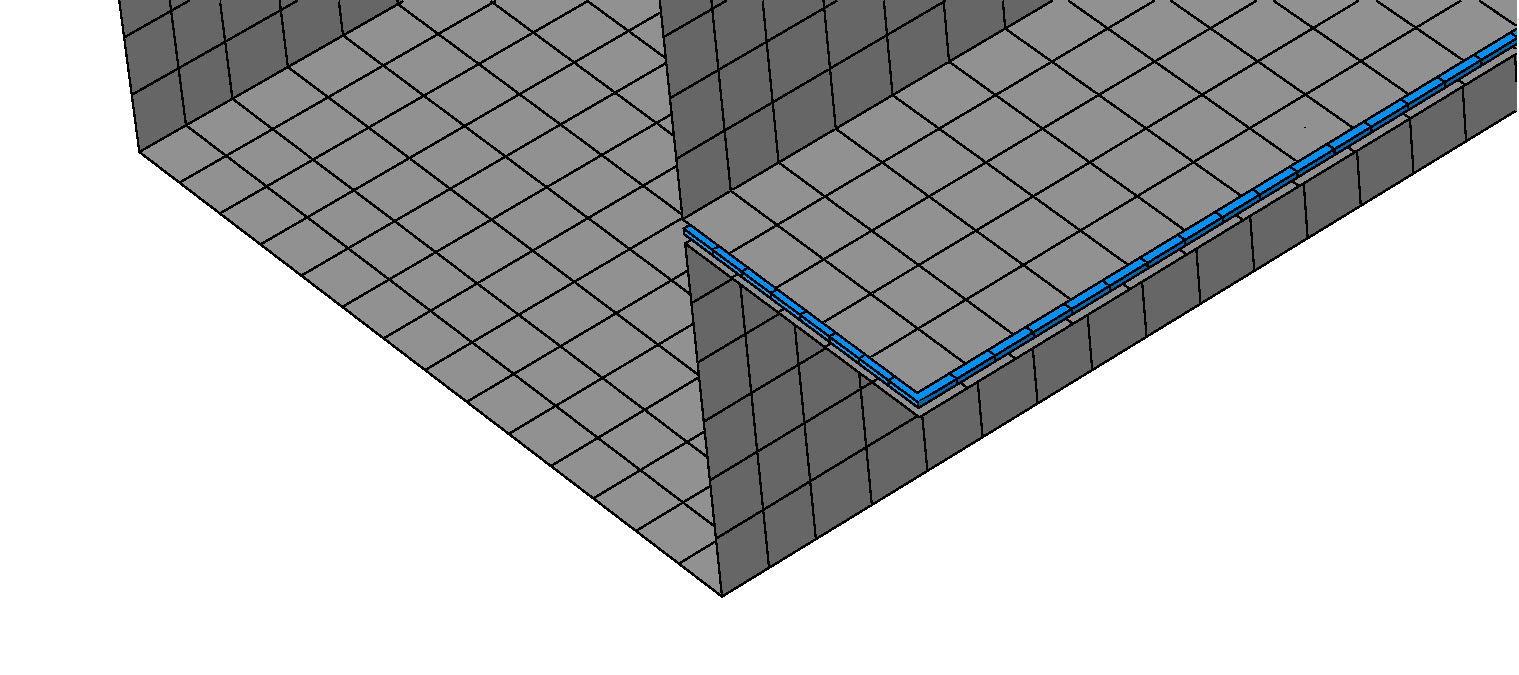
\includegraphics[width=0.7\linewidth]{figures/IMG_CUTRES/mesh_detail_coh3d_comparison}
	\caption[Detail of COH3D mesh on the adhesive layer.]{Detail of COH3D mesh on the adhesive layer (blue).}
	\label{fig:mesh_detail_coh3d_comparison}
\end{figure}

% Mesh divisions for structure
Parts were partitioned, so a structured mesh could be applied in the most of the model, and limiting free meshes to the trigger surroundings. This detail is represented in \cref{fig:mesh_part}. It was firstly considered one of reasons for critical situations, and was performed aiming to relieve a possible numerical origin of these problems. Although it was eventually proven to not be related, it was finally maintained.

\begin{figure}
	\centering
	\begin{minipage}[b]{.48\linewidth}
		\centering
		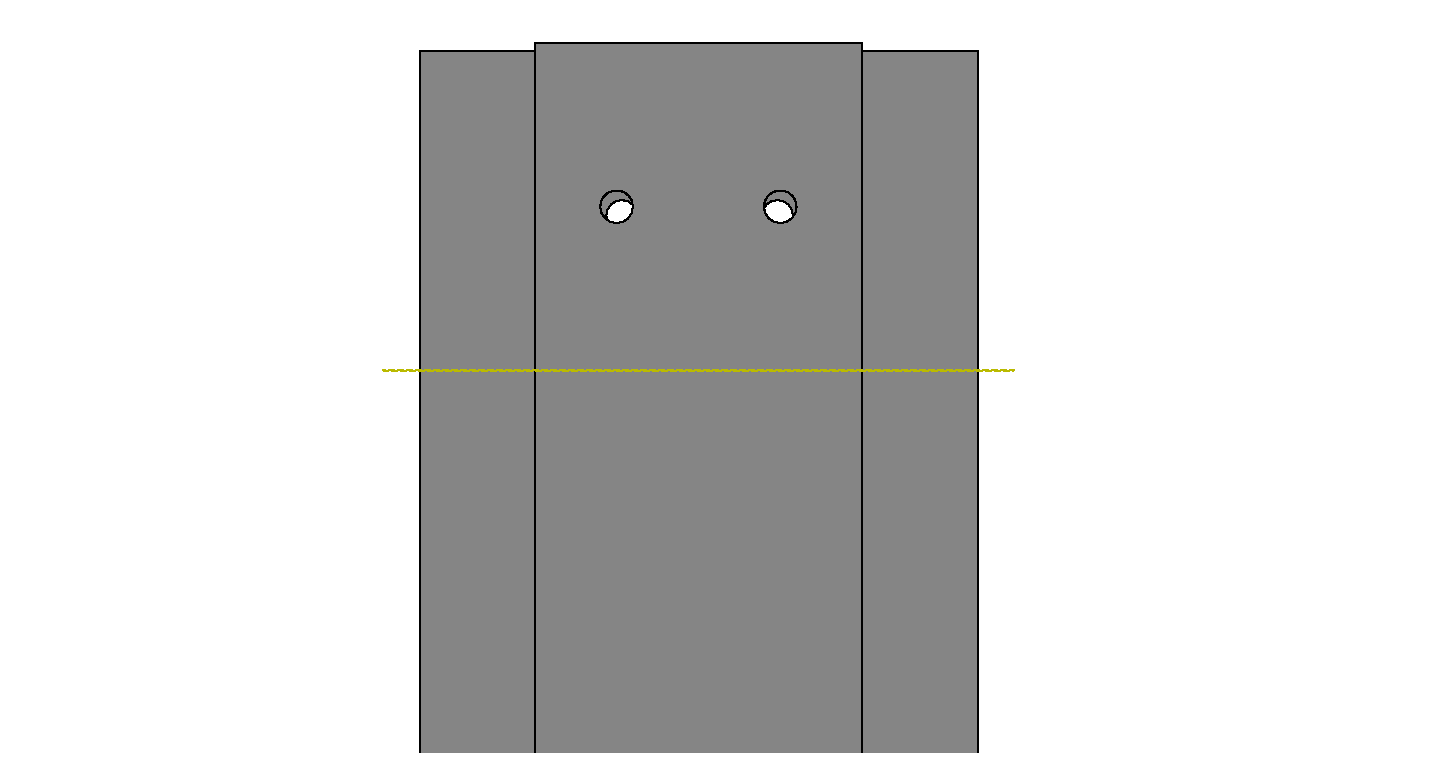
\includegraphics[width=\linewidth]{figures/IMG_CUTRES/assembly_detail_holes}
	\end{minipage}
	\quad
	\begin{minipage}[b]{.48\linewidth}
		\centering
		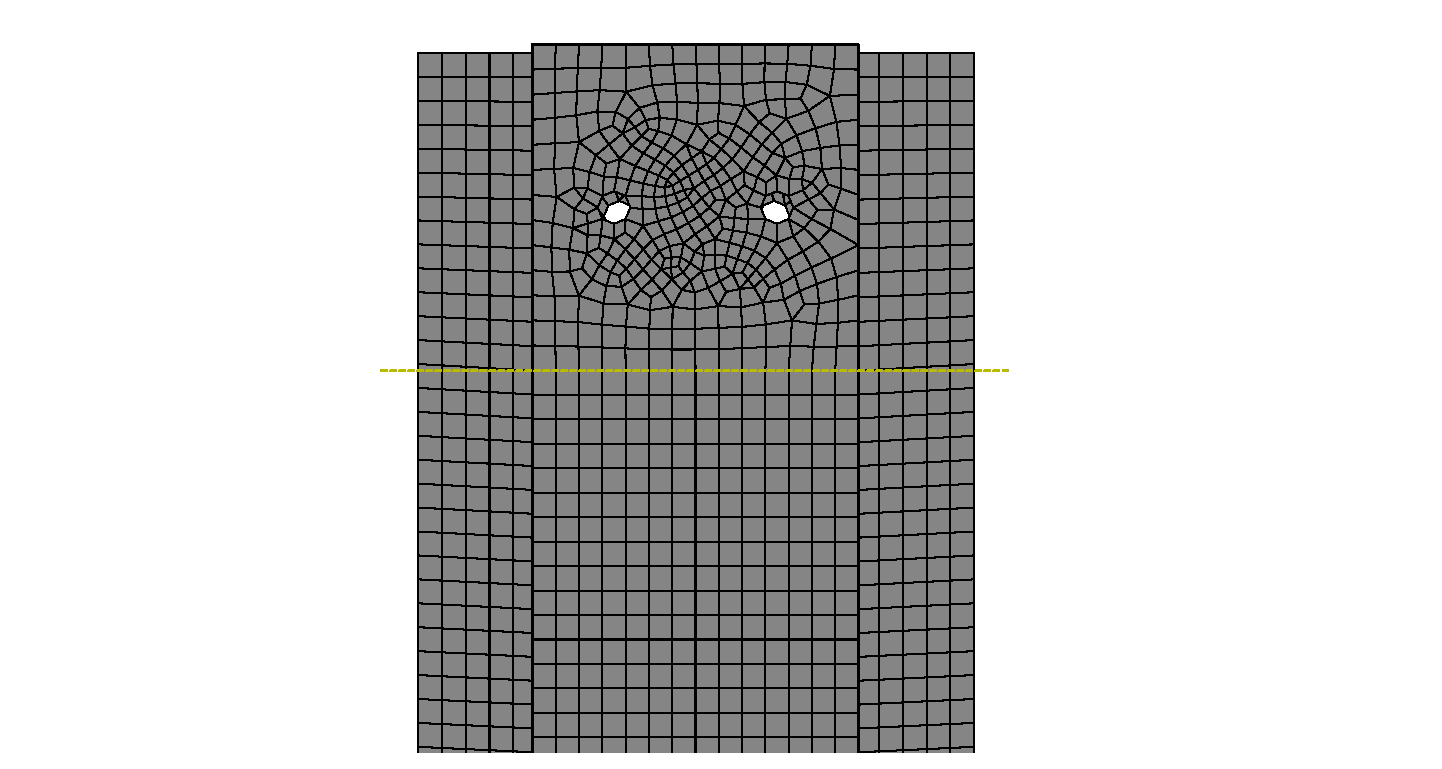
\includegraphics[width=\linewidth]{figures/IMG_CUTRES/mesh_detail_holes}
	\end{minipage}
\caption{Assembly partitions detail for mesh structuring.}
\label{fig:mesh_part}
\end{figure}

Finally, \cref{fig:mesh} shows the used mesh for the crash tube, which has more than $\num{10600}$ elements, as \cref{tab:mesh} summarizes. In that same table, different element types are mentioned: ``S3'' and ``S4R'' are three and four noded general purpouse shell elements for structural analysis (the former one also includes reduced integration); ``R3D4'' are four noded 3D rigid quadrilateral; and ``COH3D'' are explained on \cref{sec:coh_elem}.

\begin{figure}
	\centering
	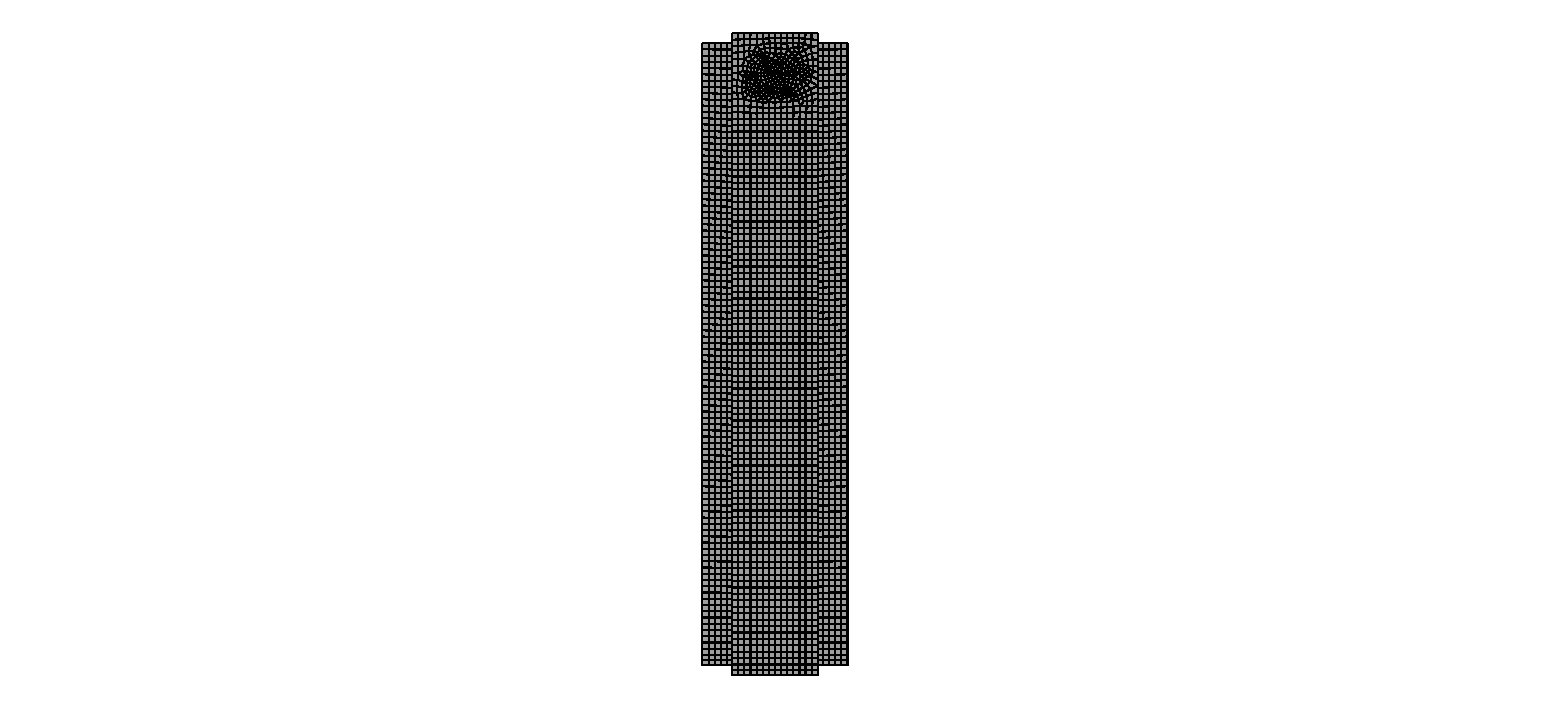
\includegraphics[width=0.9\linewidth]{figures/IMG_CUTRES/mesh}
	\caption{General mesh of the crash box.}
	\label{fig:mesh}
\end{figure}

% Total recount of elements (by part?)
\begin{table}
	\centering
	\begin{tabular}{ll p{3cm} rr}
		Part & Element type & Mesh type & Elements & Nodes \\
		Adherend & S4R (S3) & Structured (with free partitions) & $3844$ ($33$) & $4010$ \\
		Adhesive & COH3D & Structured & $1200$ & $2718$ \\
		Rigid plates & R3D4 & Free & $10$ & $15$ \\
		Stabilizing box & R3D4 & Structured & $448$ & $480$ \\
		Total &&& $10622$ & $13966$ \\
	\end{tabular}
	\caption[Mesh summary.]{Mesh summary. Given values correspond to each instance of that part. In the adherend case, there is a seven element recount difference between each instance, probably due to the free mesh control in some partitions. The average value is given.}
	\label{tab:mesh}
\end{table}


As \cite{Hale} explains, in explicit dynamic modelling, the total running time depends both on the model size (mesh size and total modelled time span) and in the time step size (${\Delta}t$). SDT is the maximum time step that still grants the numerical stability of the calculations, by supressing the possibility to a mechanical stress wave to go through more than one element in each time step. This condition is known as the Courant condition:

\begin{equation}
{\Delta}t_{stable} \leq f \left[\frac{h}{c}\right]_{min} ;
\label{eq:courant}
\end{equation}
where $f$ is a factor, usually $0.9$; $h$ is the element dimension; and $c$ is the wave speed in that same element; the minimum is calculated within the whole model. The wave speed can be calculated as

\begin{equation}
c = \sqrt{\frac{E}{\rho}} ;
\label{eq:wave_speed}
\end{equation}
where $E$ is the Young modulus; and $\rho$, the density. Among the values expresed in \cref{eq:courant,eq:wave_speed}, only density can be modified without heavily affecting accuracy. Applying this in order to improve numerical performance of the model is known as mass scaling.

Software packages calculation kernels usually include this feature applying it selectively to those elements which are determining the unfavorable SDT in each time step.

Following \cite{Scattina2011}, mass scaling was applied to the adhesive's density in the whole model, that is, with a given selection of element which corresponds to all adhesive elements.

Increasing it one order of magnitude results on a SDT up to 30 times bigger. Increasing it two orders of magnitude results in very similar improvements, a bit worse perhaps. A factor of 40 was finally used, resulting in a SDT almost two orders of magnitude bigger than the original ones.

\subsubsection{The COH3D}
\label{sec:coh_elem}

As COH3D were specifically formulated for adhesive modelling, among other uses, they have been widely used to model this material, in Abaqus \cite{Sadowski2010, Sadowski2011, Sadowski2014, Alvarez2014} and in other software packages \cite{Sato2000, Carlberger2007, Loureiro2010, Scattina2011, Ghasemnejad2013}, although this is not the only existing formulation \cite{Sato2000, Greve2007, Liao2011, Yang2012}. Certain stress distributions cannot be properly modelled, such as in-plane compression, but these have no interest or negligible effects. In Abaqus, these elements are denominated COH3D and require that:
\begin{itemize}
	\item There can only be a single layer of elements.

	\item Element's shape must be plate-like: height smaller than the other dimensions, but not negligible.

	\item A stack direction, usually based on the first point, and represented by $x'_{2}$ in \cref{fig:coh3d_csys}, in order to define the direction of the traction loading.
\end{itemize}

As the adhesive layer is very thin, it matches this geometrical requirements, making these elements suitable for this application (see \cref{fig:mesh_detail_coh3d_comparison}). These needed aspect ratios allow a coarser mesh on this part, if compared to general purpouse 3D elements, with access to better-fit formulations, and thus good results.

\begin{figure}
	\centering
	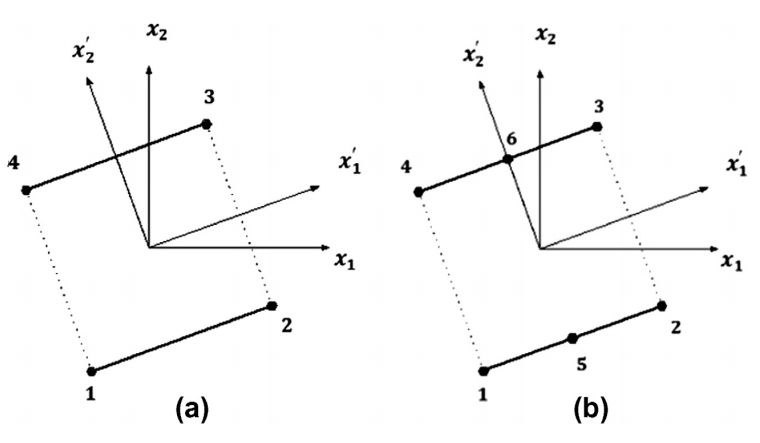
\includegraphics[width=0.7\linewidth]{figures/IMG_CUTRES/coh3d_csys}
	\caption[Representation of linear and cuadratic cohesive 2D elements.]{Representation of linear (a) and cuadratic (b) cohesive 2D elements. Axis denoted as $x_{i}$ are refered to the global coordinate system, being the $x'_{i}$ in the local coordinate system. In this case, $x'_{1}$ is the in-plane axis, and $x'_{2}$ is the normal axis, paralell to stack direction. Taken from \cite{Alvarez2014}.}
	\label{fig:coh3d_csys}
\end{figure}

COH3D with the same element length as the adherend elements could be used without computational problems. But a such coarse mesh showed some difficulties on modelling damage behaviour, depicting a too staggered failure, instead of being more continuous-like.

\begin{figure}
\centering
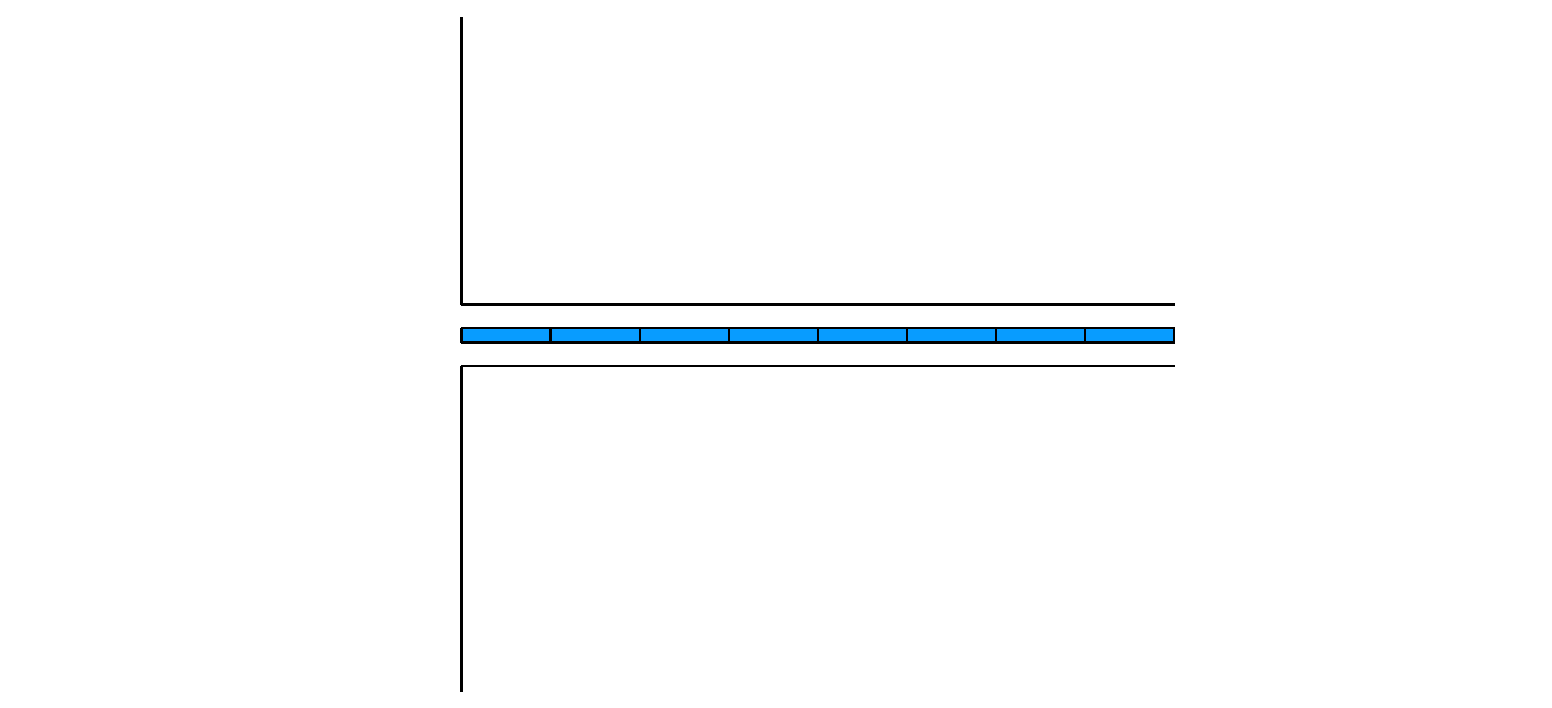
\includegraphics[width=0.7\linewidth]{figures/IMG_CUTRES/ads_detail}
\caption{Frontal detail of the adhesive layer elements.}
\label{fig:ads_detail}
\end{figure}

Although the quadratic nominal stress criterion formulation exists as a bulk damage model and as a contact damage model, only the former one was used. Using both would have been more realistic \cite{Wu2013}, but it brought simulation problems: elements separating alternatively from each adherend appeared together with elements inbetween in good state. Instead of getting stiffness degradation in the whole adhesive, undamaged elements were here subjected to the load their neighbours weren't handling, and thus failing significantly reducing adhesive's overall resistance, apart from other numerical issues.

The contact interaction was eventually substituted by a tie constraint between the COH3D surface and the adherend elements (see \cref{fig:ads_detail} for in-model detail, and \cref{fig:union} for a schematic view of the concept). It is suppossed that the use of quadratic nominal stress criterion for contact interaction properties is more suitable for those cases in which the bulk of the adhesive layer is not of interest and the focus is on a general behaviour of the structure.

\begin{figure}
	\centering
	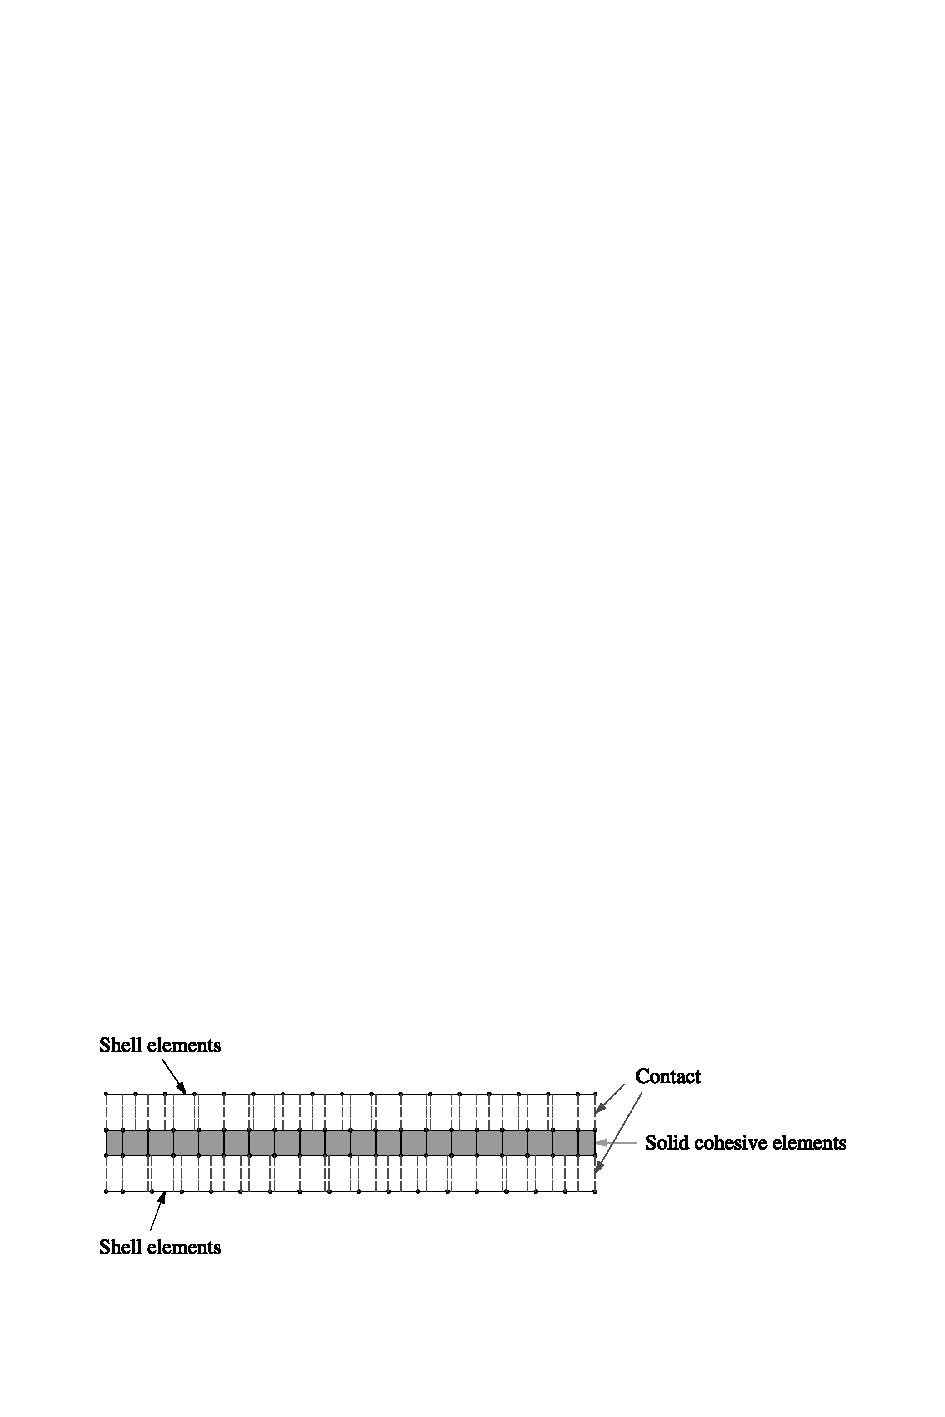
\includegraphics[width=0.7\linewidth]{figures/IMG_CUTRES/union}
	\caption[Cross section detail of the adhesive layer modelled with COH3D between two adherends modelled with shell elements.]{Cross section detail of the adhesive layer modelled with COH3D between two adherends modelled with shell elements. Taken from \cite{Scattina2011}.}
	\label{fig:union}
\end{figure}

As the used damage model is a particular case of VCCT, it can only be applied in certain element types, like the COH3D. It supposes a formulation that strongly penalizes the minimum SDT \cite{Abaqus613Manual}, reducing it even to the order of $\SI{1.5e-9}{\s}$, much more unfavorable if compared to other damage models tried during the development of this study, which made it about $\SI{2e-7}{\s}$.

It is recommended to see the work done by \cite{Alfano2001} for a deeper explanation on the COH3D element formulation, and the article written by \cite{May2014} for deeper information on failure formulations.
\todo{Poner bien las referencias (cite pero que funcione)}
\section{Optimization strategy}


\subsection{Surrogate-based methods}

In order to optimize the specimen, a surrogate-optimization approach is used. Therefore, the computationally-expensive  objective functions of the model are replaced by another functions less costly to evaluate. 

Firstly, with the parametrized model, a sampling of !!N!! samples is performed, relying on the LHS technique. This method creates a set of data with homogeneous projections on each variable axis, so that no superimposed projections appear. 

Once the sampling is obtained, the surrogate model is created. The Multivariate adaptive regression splines (MARS) method is chosen, where the surrogate functions are adjusted with cubic splines following the next expression
\begin{equation}\label{eq:mars}
\hat{f}\left ( \bm{x} \right )= \sum_{m=1}^{M}a_{m}B_{m}\left ( \bm{x} \right ),
\end{equation}
where $B_{m}$ are the power basis functions, $a_{m}$ the coefficients of the functions, and $M$ is the number of functions. This method is more thoroughly explained in \cite{Friedman1995197}. 

In order to judge the accuracy of the trend functions, the goodness of fit $R^2$, needs to be looked into. This indicator is defined as
\begin{equation}\label{eq:correlation_coefficient}
  R^2 = {\left(\dfrac{\sigma_{\bm{f}
\bm{\hat{f}}}}{\sqrt{\sigma_{\bm{f}}^2
\sigma_{\bm{\hat{f}}}^2}}\right)}^2
\end{equation}

This is done for all objective functions, where values equal or higher than $0.95$ for the selected objective functions are expected. 

With the surrogate-based model created, two optimization strategies are used. In a first approach, single-objective optimization techniques are applied. The calculations that this type of optimization requires are relatively simple once the proper surrogate model has been built. Single-objective optimization searches for the minima of the function within the limits of the design space. Traditional methods involving gradient-based and Hessian-based information are not very useful for optimizing the type of problems studied in this research, since many local minima are found in the function, yielding only misleading results. Therefore, a single-objective evolutionary algorithm is used, since this type of methods are slower but dodge local minima with ease.

The other type of optimization used is multi-objective optimization. This procedure involves more resources for the calculations. Instead of a single point, the results are conformed by a Pareto front, corresponding to a range of results. The set of all Pareto optimal design configurations, $P^*$, is defined as:

\begin{equation}
P^* := \left\{ x \in \Pi \   \nexists x' \in \Pi \    \hat{f}_i \left( \bm{x'} \right) \leqslant \hat{f}_i \left( \bm{x} \right)  \right\}
\end{equation}
and the Pareto front, which is the set of optimal objective functions from the Pareto design configurations, $PF^*$, is defined as:

\begin{equation}
PF^* := \left\{ \overline{\bm{u}} = \left( \hat{f}_1 \left( \bm{x} \right), \ldots , \hat{f}_k \left( \bm{x} \right) \right)  x \in P^* \right\}
\end{equation}

In the end, the set of points from the Pareto front has a number of components equal to the number of objective functions, each constituting a feasible solution to the problem. This Pareto front points cannot improve the value of one objective function without worsening the value of at least one other objective function.

Therefore, the results shall be analyzed and, depending on the needs required for the specimen, one or other point on the frontier is chosen. As with the single-objective optimization, multi-objective optimization usually has problems with local minima. For this problem, genetic algorithms are used, aiming for better and more reliable results.

The methods selected for both the single- and the multi-objective optimization are the genetic algorithms from the JEGA Library, developed by \cite{JEGA}. This methods perform optimization supporting general constraints as well as mixtures of real and discrete variables. The variables are encoded and referred to as chromosomes, and each digit of the variable is a gene.

\subsection{Metrics}

The objective of this research is to find a set of optimum designs of the specimen previously described according to three different objective functions. These functions are the absorbed energy ($E_a$), the mass of the specimen ($m$) and the peak load ($P_{peak}$). The three metrics are obtained using a finite element simulation, where $E_a$ and $P_{peak}$ are obtained via the force-displacement curves.

Before making any calculations with the force-displacement curve, and according to the specialized literature in crash analysis \cite{Huanglibro}, a standard SAE 600 filter \cite{J211} is applied. This removes the high-frequency noise from the curve with a cutoff frequency of ${1000}$ Hz. Once the filter is used, the direct integration of the resulting force-displacement curve yields to the $E_a$:
\begin{equation}\label{Ea}
  E_{a}=\int _{0}^{\delta }F\! \left( z \right) \,dz\,,
\end{equation}
with $\delta$ being the total axial crushing distance and $F\! \left( z \right)$ the value of the crushing force at the crushing length $z$.

The peak load $P_{peak}$ is defined as
\begin{equation}\label{Peak}
 P_{peak}=max\left\{ F\! \left( z \right)  \forall z \in [0,\delta] \right\}
\end{equation}

These three objective functions have not been randomly chosen. The first reason is the nature of the design and its aim to improve the crashworthiness of vehicles. The $E_a$ can be easily improved by increasing the thicknesses of the materials, but this would harm the other two objective functions $m$ and $P_{peak}$, increasing both of them. An increase in the mass of the specimen translates into a higher mass of the vehicle, increasing its fuel consumption and reducing its performance; whereas an increase in the $P_{peak}$ means a higher force and acceleration suffered by the passengers of the vehicle, raising the odds of resulting in a serious injury.

The second reason for choosing these objective functions is purely computational. Traditionally, other researchers have swerved towards optimization of the specific energy absorption (SEA) and the load ratio (LR) \cite{Hou2007555}. The SEA function is defined as a ratio between $E_a$ and $m$:
\begin{equation}\label{SEA}
  S\! EA=\dfrac {E_a} {m}
\end{equation}

By contrast, the load ratio relates the $P_{peak}$ with the mean load $P_m$ as
\begin{equation}\label{LR}
  LR=\dfrac {P_{peak}} {P_m}
\end{equation}

The mean load is obtained as a ratio between the absorbed energy and the total crushing length $\delta$:
\begin{equation}\label{Pm}
  P_{m}=\dfrac {E_a} {\delta}
\end{equation}

The SEA and LR were also evaluated as objective functions, but it was found that during the optimization process these quantities have a more complicated comportment and a noisier nature for this model. Consequently, they were only used during the parameter study and the single-objective optimization. They were discarded from the multi-objective  optimization process and are only used as indicators to compare different specimens.

The peak load is also used as a constraint in the single-objective optimization. This is done so that, in the real specimen, the required force to crumple the piece is never over a certain value, thus protecting the rest of the car's chassis and the occupants. In the multi-objective optimization this is not required nor used, since the final results consist of Pareto fronts, where the maximum peak load depends on the mass or energy absorption desired.

\subsection{Optimization process}

In order to optimize the model, the process has been divided into different stages. Firstly, a parameter study is performed. A simple sampling of the work space for each variable is carried out. With this, a general idea of the variables' behavior is obtained.

Secondly, single-objective optimization is run for the SEA objective function. Whereas an optimization of the mass and the absorbed energy would provide better results, this can be easier optimized, since the other option requires multi-objective optimization. Both unconstrained and constrained optimization procedures are considered, setting a limit for the peak load constraint in the latter.

Lastly, multi-objective unconstrained optimization is sought. All objective functions are minimized, and the points obtained as solution cannot be improved in a variable without harming, at least, another one. This last step is the most complete, giving more information of the behavior of the functions and the optimization process, but due to the greater complexity in the evaluation it is computed the last.


\section{Conclusions}
\todo{Quitar el usepackage todonotes}
\section{Acknowledgments}



\bibliography{./references/references}

\end{document}
